\section{прямые на координатной плоскости решения}
1. Так как при больших положительных значениях $x$ значения $y$ будут положительны, $k>0.$ Подставим в уравнение прямой точку $(1;b):\ b=k\cdot1+b \Rightarrow k=0,$ что противоречит тому, что $k>0.$ Теперь подставим в уравнение прямой все значения из пункта в): $-1,38=\cfrac{1}{2}\cdot1,22-2\Rightarrow-1,38=-1,39.$ Полученное равенство неверно, значит график функции через данную точку не проходит.\\
2. Так как при больших положительных значениях $x$ значения $y$ будут отрицательны, $k<0.$ Подставим в уравнение прямой точку $(1;b):\ b=k\cdot(-1)+b \Rightarrow k=0,$ что противоречит тому, что $k<0.$ Теперь подставим в уравнение прямой все значения из пункта в): $3,47=2\cdot1,73+1\Rightarrow3,47=4,46.$ Полученное равенство неверно, значит график функции через данную точку не проходит.\\
3. Если точка пересечения имеет абсциссу 8, то при подстановке $x=8$ в оба уравнения прямых должно получиться одно и то же число, то есть
$\cfrac{1}{4}\cdot8+3a=\cfrac{1}{2}\cdot8-a,\ 2+3a=4-a,\ 4a=2,\ a=\cfrac{1}{2}.$\\
4. Если точка пересечения имеет абсциссу 3, то при подстановке $x=3$ в оба уравнения прямых должно получиться одно и то же число, то есть
$\cfrac{1}{3}\cdot3+2p=\cfrac{1}{2}\cdot3+p,\ 1+2p=\cfrac{3}{2}+p,\ p=\cfrac{1}{2}.$\\
5. $(x-5)(2y+4x-6)=0\Leftrightarrow\left[\begin{array}{c}x-5=0,\\ 2y+4x-6=0.\end{array}\right.\Leftrightarrow\left[\begin{array}{c}x=5,\\ y=3-2x.\end{array}\right.$
$$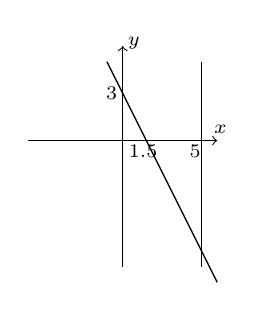
\begin{tikzpicture}[scale=0.2]
\tikzset {line01/.style={line width =0.5pt}}
\tikzset{line02/.style={line width =1pt}}
\tikzset{line03/.style={dashed,line width =0.5pt}}
%\filldraw [black] (0,0) circle (1pt);
\draw [->] (-6,0) -- (6,0);
\draw [->] (0,-8) -- (0,6);
\draw[line01] (5,-8) -- (5,5);
\draw[line01] (-1,5) -- (6,-9);
\draw (6.2,0.7) node {\scriptsize $x$};
\draw (4.6,-0.7) node {\scriptsize $5$};
\draw (1.3,-0.7) node {\scriptsize $1.5$};
\draw (-0.7,3) node {\scriptsize $3$};
\draw (0.7,6.2) node {\scriptsize $y$};
\end{tikzpicture}$$
6. $(x+4)(3y-6x+9)=0\Leftrightarrow\left[\begin{array}{c}x+4=0,\\ 3y-6x+9=0.\end{array}\right.\Leftrightarrow\left[\begin{array}{c}x=-4,\\ y=2x-3.\end{array}\right.$
$$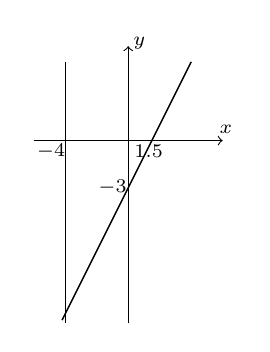
\begin{tikzpicture}[scale=0.2]
\tikzset {line01/.style={line width =0.5pt}}
\tikzset{line02/.style={line width =1pt}}
\tikzset{line03/.style={dashed,line width =0.5pt}}
%\filldraw [black] (0,0) circle (1pt);
\draw [->] (-6,0) -- (6,0);
\draw [->] (0,-11.6) -- (0,6);
\draw[line01] (-4,-11.6) -- (-4,5);
\draw[line01] (4,5) -- (-4.2,-11.4);
\draw (6.2,0.7) node {\scriptsize $x$};
\draw (-4.9,-0.7) node {\scriptsize $-4$};
\draw (1.3,-0.7) node {\scriptsize $1.5$};
\draw (-1,-3) node {\scriptsize $-3$};
\draw (0.7,6.2) node {\scriptsize $y$};
\end{tikzpicture}$$
7. Если все три прямые пересекаются в одной точке, то в ней должны выполняться все три равенства, так что подставим $y=2x+1$ в первые два уравнения:
$\begin{cases} x=a-3(2x+1),\\ 2(2x+1)=5-a-3x.\end{cases}\Leftrightarrow\begin{cases} x=a-6x-3,\\ 4x+2=5-a-3x.\end{cases}\Leftrightarrow
\begin{cases} 7x-a=-3,\\ 7x+a=3.\end{cases}\Rightarrow 2a=6 \Rightarrow a=3.$\\
8. Если все три прямые пересекаются в одной точке, то в ней должны выполняться все три равенства, так что подставим $y=x-8$ в первые два уравнения:
$\begin{cases} x=2(x-8)+b,\\ 3(x-8)=b-1+x.\end{cases}\Leftrightarrow$\\$\begin{cases} x=2x-16+b,\\ 3x-24=b-1+x.\end{cases}\Leftrightarrow
\begin{cases} -x-b=-16,\\ 2x-b=23.\end{cases}\Leftrightarrow
\begin{cases} -2x-2b=-32,\\ 2x-b=23.\end{cases}\Rightarrow -3b=-9 \Rightarrow b=3.$\\
9. Эта прямая при любом $k$ проходит через точку $(0;4),$ то есть один из катетов отсекаемого прямоугольного треугольника равен 4. Если второй катет тоже равен 4 и отсекаемый треугольник находится в I четверти, она должна проходить также через точку $(4;0),$ поэтому $0=k\cdot4+4,\ k=-1.$\\
10. Эта прямая при любом $k$ проходит через точку $(0;5),$ то есть один из катетов отсекаемого прямоугольного треугольника равен 5. Если второй катет тоже равен 5 и отсекаемый треугольник находится в I четверти, она должна проходить также через точку $(5;0),$ поэтому $0=k\cdot5+5,\ k=-1.$\\
11. а) Подставим координаты точки $A$ в уравнение: $1196=239k+1,\ k=5.$ Построим график прямой $y=5x+1$ по двум точкам $(0;1)$ и $(1;6).$
$$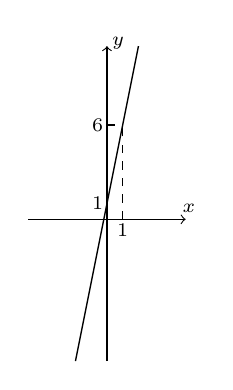
\begin{tikzpicture}[scale=0.2]
\tikzset {line01/.style={line width =0.5pt}}
\tikzset{line02/.style={line width =1pt}}
\tikzset{line03/.style={dashed,line width =0.5pt}}
%\filldraw [black] (0,0) circle (1pt);
\draw [->] (-5,0) -- (5,0);
\draw [->] (0,-9) -- (0,11);
\draw[line01] (-2,-9) -- (2,11);
\draw[line03] (1,0) -- (1,6);
\draw[line03] (0,6) -- (1,6);
\draw (5.2,0.7) node {\scriptsize $x$};
\draw (-0.6,1) node {\scriptsize $1$};
\draw (-0.6,6) node {\scriptsize $6$};
\draw (1,-0.7) node {\scriptsize $1$};
\draw (0.7,11.2) node {\scriptsize $y$};
\end{tikzpicture}$$
б) Эта прямая при любом $k$ проходит через точку $(0;1),$ то есть один из катетов отсекаемого прямоугольного треугольника равен 1. Если второй катет отличается от него в 5 раз, то возможны 4 случая: он больше в 5 раз и точка пересечения с осью абсцисс имеет положительное или отрицательное значение или он меньше в 5 раз и точка пересечения с осью абсцисс имеет положительное или отрицательное значение. Таким образом, искомая прямая должна проходить через одну из точек $(5;0),\ (-5;0),\ \left(\cfrac{1}{5};0\right),\ \left(-\cfrac{1}{5};0\right).$ Подставим эти точки в уравнение прямой и найдём все возможные значения $k:\ 5k+1=0,\ k=-\cfrac{1}{5};\ -5k+1=0,\ k=\cfrac{1}{5};\ \cfrac{1}{5}k+1=0,\ k=-5;\ -\cfrac{1}{5}k+1=0,\ k=5.$\\
12. а) Подставим координаты точки $B$ в уравнение: $239=79a+2,\ a=3.$ Построим график прямой $y=3x+2$ по двум точкам $(0;2)$ и $(1;5).$
$$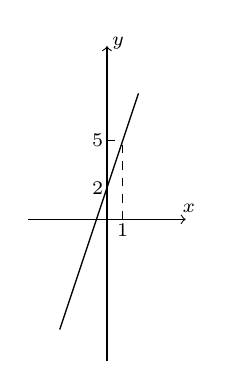
\begin{tikzpicture}[scale=0.2]
\tikzset {line01/.style={line width =0.5pt}}
\tikzset{line02/.style={line width =1pt}}
\tikzset{line03/.style={dashed,line width =0.5pt}}
%\filldraw [black] (0,0) circle (1pt);
\draw [->] (-5,0) -- (5,0);
\draw [->] (0,-9) -- (0,11);
\draw[line01] (-3,-7) -- (2,8);
\draw[line03] (1,0) -- (1,5);
\draw[line03] (0,5) -- (1,5);
\draw (5.2,0.7) node {\scriptsize $x$};
\draw (-0.6,2) node {\scriptsize $2$};
\draw (-0.6,5) node {\scriptsize $5$};
\draw (1,-0.7) node {\scriptsize $1$};
\draw (0.7,11.2) node {\scriptsize $y$};
\end{tikzpicture}$$
б) Эта прямая при любом $a$ проходит через точку $(0;2),$ то есть один из катетов отсекаемого прямоугольного треугольника равен 2. Если второй катет отличается от него в 1,5 раз, то возможны 4 случая: он больше в 1,5 раза и точка пересечения с осью абсцисс имеет положительное или отрицательное значение или он меньше в 1,5 раза и точка пересечения с осью абсцисс имеет положительное или отрицательное значение. Таким образом, искомая прямая должна проходить через одну из точек $(3;0),\ (-3;0),\ \left(\cfrac{4}{3};0\right),\ \left(-\cfrac{4}{3};0\right).$ Подставим эти точки в уравнение прямой и найдём все возможные значения $k:\ 3a+2=0,\ a=-\cfrac{2}{3};\ -3a+2=0,\ a=\cfrac{2}{3};\ \cfrac{4}{3}a+2=0,\ a=-\cfrac{3}{2};\ -\cfrac{4}{3}a+2=0,\ a=\cfrac{3}{2}.$\\
13. а) Построим искомый треугольник по точкам пересечения данных прямых с осями координат: $(-3;0),\ (0;2),\ (0;-2).$
$$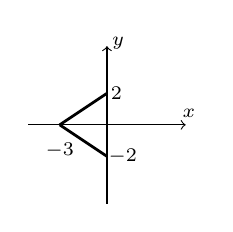
\begin{tikzpicture}[scale=0.2]
\tikzset {line01/.style={line width =0.5pt}}
\tikzset{line02/.style={line width =1pt}}
\tikzset{line03/.style={dashed,line width =0.5pt}}
%\filldraw [black] (0,0) circle (1pt);
\draw [->] (-5,0) -- (5,0);
\draw [->] (0,-5) -- (0,5);
\draw[line02] (-3,0) -- (0,2);
\draw[line02] (-3,0) -- (0,-2);
\draw[line02] (0,2) -- (0,-2);
\draw (5.2,0.7) node {\scriptsize $x$};
\draw (0.6,2) node {\scriptsize $2$};
\draw (1,-2) node {\scriptsize $-2$};
\draw (-3,-1.6) node {\scriptsize $-3$};
\draw (0.7,5.2) node {\scriptsize $y$};
\end{tikzpicture}$$
б) Все прямые вида $y=-x+b$ параллельны друг другу. Самая нижняя из них проходит через точку $(-3;0),$ поэтому $0=3+b,\ b=-3$ --- наименьшее подходящее значение. Самая верхняя из них проходят через точку $(0;2),$ поэтому $2=0+b,\ b=2$ --- наибольшее подходящее значение. Таким образом, $-3\leqslant b \leqslant 2.$\\
14. а) Построим искомый треугольник по точкам пересечения данных прямых с осями координат: $(3;0),\ (0;2),\ (0;-2).$
$$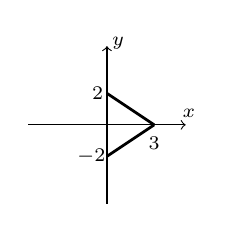
\begin{tikzpicture}[scale=0.2]
\tikzset {line01/.style={line width =0.5pt}}
\tikzset{line02/.style={line width =1pt}}
\tikzset{line03/.style={dashed,line width =0.5pt}}
%\filldraw [black] (0,0) circle (1pt);
\draw [->] (-5,0) -- (5,0);
\draw [->] (0,-5) -- (0,5);
\draw[line02] (3,0) -- (0,2);
\draw[line02] (3,0) -- (0,-2);
\draw[line02] (0,2) -- (0,-2);
\draw (5.2,0.7) node {\scriptsize $x$};
\draw (-0.6,2) node {\scriptsize $2$};
\draw (-1,-2) node {\scriptsize $-2$};
\draw (3,-1.2) node {\scriptsize $3$};
\draw (0.7,5.2) node {\scriptsize $y$};
\end{tikzpicture}$$
б) Все прямые вида $y=-x+b$ параллельны друг другу. Самая нижняя из них проходит через точку $(0;-2),$ поэтому $-2=0+b,\ b=-2$ --- наименьшее подходящее значение. Самая верхняя из них проходят через точку $(3;0),$ поэтому $0=-3+b,\ b=3$ --- наибольшее подходящее значение. Таким образом, $-2\leqslant b \leqslant 3.$\\
15. Составим и решим систему уравнений: $\begin{cases} 4k+b=-6,\\ -8k+b=-12.\end{cases}\Rightarrow 12k=6\Rightarrow k=\cfrac{1}{2}\Rightarrow b=-8.$
Преобразуем прямую $2x+y=2$ в $y=2-2x$ и приравняем правые части: $2-2x=\cfrac{1}{2}x-8,\ -\cfrac{5}{2}x=-10,\ x=4,\ y=2-2\cdot4=-6.$\\
16. Составим и решим систему уравнений: $\begin{cases} 2k+b=1,\\ -4k+b=10.\end{cases}\Rightarrow 6k=-9\Rightarrow k=-\cfrac{3}{2}\Rightarrow b=4.$
Преобразуем прямую $3x-y=5$ в $y=3x-5$ и приравняем правые части: $3x-5=-\cfrac{3}{2}x+4,\ \cfrac{9}{2}x=9,\ x=2,\ y=3\cdot2-5=1.$\\
17. Построим по двум точкам $(0;-3)$ и $\left(\cfrac{3}{4};0\right)$ график функции $y=4x-3$ и отразим его вверх симметрично относительно оси абсцисс.
$$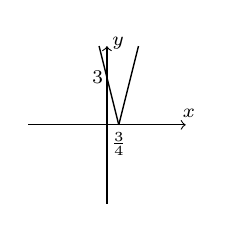
\begin{tikzpicture}[scale=0.2]
\tikzset {line01/.style={line width =0.5pt}}
\tikzset{line02/.style={line width =1pt}}
\tikzset{line03/.style={dashed,line width =0.5pt}}
%\filldraw [black] (0,0) circle (1pt);
\draw [->] (-5,0) -- (5,0);
\draw [->] (0,-5) -- (0,5);
\draw[line01] (0.75,0) -- (2,5);
\draw[line01] (0.75,0) -- (-0.5,5);
\draw (5.2,0.7) node {\scriptsize $x$};
\draw (-0.6,3) node {\scriptsize $3$};
\draw (0.75,-1.2) node {\scriptsize $\frac{3}{4}$};
\draw (0.7,5.2) node {\scriptsize $y$};
\end{tikzpicture}$$
18. Построим по двум точкам $(0;-3)$ и $\left(\cfrac{3}{4};0\right)$ график функции $y=4x-3$ и отразим его влево симметрично относительно оси ординат.
$$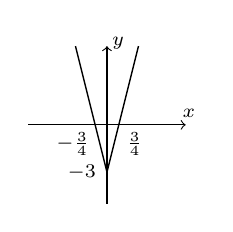
\begin{tikzpicture}[scale=0.2]
\tikzset {line01/.style={line width =0.5pt}}
\tikzset{line02/.style={line width =1pt}}
\tikzset{line03/.style={dashed,line width =0.5pt}}
%\filldraw [black] (0,0) circle (1pt);
\draw [->] (-5,0) -- (5,0);
\draw [->] (0,-5) -- (0,5);
\draw[line01] (0,-3) -- (2,5);
\draw[line01] (0,-3) -- (-2,5);
\draw (5.2,0.7) node {\scriptsize $x$};
\draw (-1.6,-3) node {\scriptsize $-3$};
\draw (1.75,-1.2) node {\scriptsize $\frac{3}{4}$};
\draw (-2.15,-1.2) node {\scriptsize $-\frac{3}{4}$};
\draw (0.7,5.2) node {\scriptsize $y$};
\end{tikzpicture}$$
19. Составим и решим систему уравнений: $\begin{cases} 3k+b=9,\\ -6k+b=-9.\end{cases}\Rightarrow 9k=18\Rightarrow k=2\Rightarrow b=3.$ Найдём точку пересечения, приравняв значение $y$ к $6:\ 2x+3=6,\ x=\cfrac{3}{2}.$\\
20. Составим и решим систему уравнений: $\begin{cases} 3k+b=9,\\ -2k+b=-6.\end{cases}\Rightarrow 5k=15\Rightarrow k=3\Rightarrow b=0.$ Найдём точку пересечения, приравняв значение $y$ к $-3:\ 3x=-3,\ x=-1.$\\
21. Так как прямые идут <<вправо--вверх>>, значения $k_1$ и $k_2$ положительны, при этом наклон прямой $l_2$ круче, значит $k_2>k_1.$ Так как точки пересечения прямых с осью ординат расположены выше оси абсцисс, значения $b_1$ и $b_2$ положительны, при этом точка пересечения прямой $l_2$ находится выше, значит $b_2>b_1.$ Таким образом, $k_2b_2>k_1b_1.$\\
22. Так как прямые идут <<вправо--вниз>>, значения $k_1$ и $k_2$ отрицательны. Точка пересечения прямой $l_1$ с осью ординат находится выше оси абсцисс, а прямой $l_2$ --- ниже, поэтому $b_1>0,\ b_2<0.$ Таким образом, $k_2b_2>0>k_1b_1.$\\
23. Построим график по двум точкам $(-1;2)$ и $(0;-1).$
$$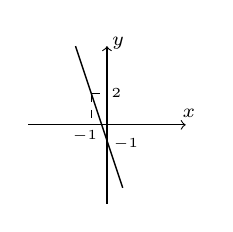
\begin{tikzpicture}[scale=0.2]
\tikzset {line01/.style={line width =0.5pt}}
\tikzset{line02/.style={line width =1pt}}
\tikzset{line03/.style={dashed,line width =0.5pt}}
%\filldraw [black] (0,0) circle (1pt);
\draw [->] (-5,0) -- (5,0);
\draw [->] (0,-5) -- (0,5);
\draw[line01] (-2,5) -- (1,-4);
\draw[line03] (-1,2) -- (-1,0);
\draw[line03] (-1,2) -- (0,2);
%\draw[line01] (0,-3) -- (-2,5);
\draw (0.6,2) node {\tiny $2$};
\draw (-1.4,-0.7) node {\tiny $-1$};
\draw (5.2,0.7) node {\scriptsize $x$};
\draw (1.2,-1.2) node {\tiny $-1$};
\draw (0.7,5.2) node {\scriptsize $y$};
\end{tikzpicture}$$
Значение $y=2$ достигается при $x=-1,$ а так как функция убывает, неравенство $y\leqslant2$ выполняется при $x\geqslant-1.$\\
24. Построим график по двум точкам $(-1;1)$ и $(0;-4).$
$$\begin{tikzpicture}[scale=0.2]
\tikzset {line01/.style={line width =0.5pt}}
\tikzset{line02/.style={line width =1pt}}
\tikzset{line03/.style={dashed,line width =0.5pt}}
%\filldraw [black] (0,0) circle (1pt);
\draw [->] (-10,0) -- (10,0);
\draw [->] (0,-10) -- (0,10);
\draw[line01] (1,-9) -- (-2,6);
\draw[line03] (-1,1) -- (0,1);
\draw[line03] (-1,0) -- (-1,1);
%\draw[line01] (0,-3) -- (-2,5);
\draw (0.6,-4) node {\tiny $-4$};
\draw (-1.6,-0.7) node {\tiny $-1$};
\draw (10.2,0.7) node {\scriptsize $x$};
\draw (0.7,1) node {\tiny $1$};
\draw (0.7,10.2) node {\scriptsize $y$};
\end{tikzpicture}$$
Значение $y=16$ достигается при $x=-4,$ а так как функция убывает, неравенство $y\geqslant16$ выполняется при $x\leqslant-4.$\\
25. $\cfrac{(x^2-9)(y+x-1)}{x-3}=0\Leftrightarrow\cfrac{(x-3)(x+3)(y+x-1)}{x-3}=0\Leftrightarrow
\begin{cases}\left[\begin{array}{l}x=-3,\\ y=1-x.\end{array}\right.\\ x\neq3\end{cases}$
$$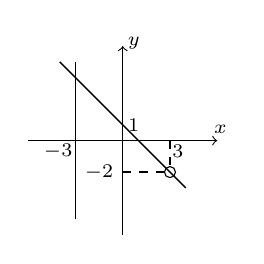
\begin{tikzpicture}[scale=0.2]
\tikzset {line01/.style={line width =0.5pt}}
\tikzset{line02/.style={line width =1pt}}
\tikzset{line03/.style={dashed,line width =0.5pt}}
%\filldraw [black] (0,0) circle (1pt);
\draw [->] (-6,0) -- (6,0);
\draw [->] (0,-6) -- (0,6);
\draw[line01] (-3,-5) -- (-3,5);
\draw[line01] (-4,5) -- (4,-3);
\draw (6.2,0.7) node {\scriptsize $x$};
\draw (-4.1,-0.7) node {\scriptsize $-3$};
\draw (3.5,-0.7) node {\scriptsize $3$};
\draw (0.7,1) node {\scriptsize $1$};
\draw (-1.5,-2) node {\scriptsize $-2$};
\draw[line03] (3,0) -- (3,-2);
\draw[line03] (0,-2) -- (3,-2);
\draw (0.7,6.2) node {\scriptsize $y$};
\draw (3,-2) circle (10pt);
\end{tikzpicture}$$
26. $\cfrac{(x^2-4)(y-x+1)}{x-2}=0=0\Leftrightarrow\cfrac{(x-2)(x+2)(y-x+1)}{x-2}=0\Leftrightarrow
\begin{cases}\left[\begin{array}{l}x=-2,\\ y=x-1.\end{array}\right.\\ x\neq2\end{cases}$
$$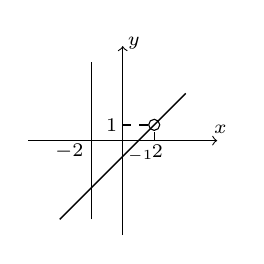
\begin{tikzpicture}[scale=0.2]
\tikzset {line01/.style={line width =0.5pt}}
\tikzset{line02/.style={line width =1pt}}
\tikzset{line03/.style={dashed,line width =0.5pt}}
%\filldraw [black] (0,0) circle (1pt);
\draw [->] (-6,0) -- (6,0);
\draw [->] (0,-6) -- (0,6);
\draw[line01] (-2,-5) -- (-2,5);
\draw[line01] (-4,-5) -- (4,3);
\draw (6.2,0.7) node {\scriptsize $x$};
\draw (-3.4,-0.7) node {\scriptsize $-2$};
\draw (2.2,-0.7) node {\scriptsize $2$};
\draw (-0.7,1) node {\scriptsize $1$};
\draw (1.1,-1) node {\tiny $-1$};
\draw[line03] (2,0) -- (2,1);
\draw[line03] (0,1) -- (2,1);
\draw (0.7,6.2) node {\scriptsize $y$};
\draw (2,1) circle (10pt);
\end{tikzpicture}$$
27. Чтобы $k$ сократилось, необходимо взять $x=-1,$ в таком случае $y=2.$\\
28. Чтобы $k$ сократилось, необходимо взять $x=1,$ в таком случае $y=1.$\\
29. а) Построим график по двум точкам $(0;3)$ и $\left(\cfrac{3}{2};0\right).$
$$\begin{tikzpicture}[scale=0.2]
\tikzset {line01/.style={line width =0.5pt}}
\tikzset{line02/.style={line width =1pt}}
\tikzset{line03/.style={dashed,line width =0.5pt}}
%\filldraw [black] (0,0) circle (1pt);
\draw [->] (-10,0) -- (10,0);
\draw [->] (0,-10) -- (0,10);
\draw[line01] (4,-5) -- (-3,9);
%\draw[line03] (-1,1) -- (0,1);
%\draw[line03] (-1,0) -- (-1,1);
%\draw[line01] (0,-3) -- (-2,5);
%\draw (0.6,-4) node {\tiny $-4$};
%\draw (-1.6,-0.7) node {\tiny $-1$};
\draw (10.2,0.7) node {\scriptsize $x$};
\draw (0.7,3) node {\tiny $3$};
\draw (1.9,0.9) node {\tiny $\frac{3}{2}$};
\draw (0.7,10.2) node {\scriptsize $y$};
\end{tikzpicture}$$
б) $-239=3-2x,\ x=121,\ 121=11^2\text{ или } (-11)^2.$\\
30. а) Построим график по двум точкам $(0;-3)$ и $\left(\cfrac{3}{2};0\right).$
$$\begin{tikzpicture}[scale=0.2]
\tikzset {line01/.style={line width =0.5pt}}
\tikzset{line02/.style={line width =1pt}}
\tikzset{line03/.style={dashed,line width =0.5pt}}
%\filldraw [black] (0,0) circle (1pt);
\draw [->] (-10,0) -- (10,0);
\draw [->] (0,-10) -- (0,10);
\draw[line01] (4,5) -- (-3,-9);
%\draw[line03] (-1,1) -- (0,1);
%\draw[line03] (-1,0) -- (-1,1);
%\draw[line01] (0,-3) -- (-2,5);
%\draw (0.6,-4) node {\tiny $-4$};
%\draw (-1.6,-0.7) node {\tiny $-1$};
\draw (10.2,0.7) node {\scriptsize $x$};
\draw (-1,-3) node {\tiny $-3$};
\draw (1.9,-0.9) node {\tiny $\frac{3}{2}$};
\draw (0.7,10.2) node {\scriptsize $y$};
\end{tikzpicture}$$
б) $239=2x-3,\ x=121,\ 121=11^2\text{ или } (-11)^2.$\\
31. а) Раз прямые параллельны, $k=3,6.$ Подставим координаты точки $D:\ 8,2=3,6\cdot(-0,5)+b,\ b=10.$  Построим прямую $y=3,6x+10$ по двум точкам $(0;10)$ и $(-5;-8).$
$$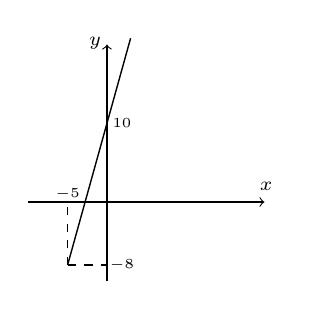
\begin{tikzpicture}[scale=0.1]
\tikzset {line01/.style={line width =0.5pt}}
\tikzset{line02/.style={line width =1pt}}
\tikzset{line03/.style={dashed,line width =0.5pt}}
%\filldraw [black] (0,0) circle (1pt);
\draw [->] (-10,0) -- (20,0);
\draw [->] (0,-10) -- (0,20);
\draw[line01] (-5,-8) -- (3,20.8);
\draw[line03] (-5,-8) -- (0,-8);
\draw[line03] (-5,-8) -- (-5,0);
%\draw[line03] (-1,1) -- (0,1);
%\draw[line03] (-1,0) -- (-1,1);
%\draw[line01] (0,-3) -- (-2,5);
%\draw (0.6,-4) node {\tiny $-4$};
%\draw (-1.6,-0.7) node {\tiny $-1$};
\draw (20.2,2) node {\scriptsize $x$};
\draw (-5,1) node {\tiny $-5$};
\draw (1.9,-8) node {\tiny $-8$};
\draw (1.9,10) node {\tiny $10$};
\draw (-1.5,20.2) node {\scriptsize $y$};
\end{tikzpicture}$$
б) Подходят любые две прямые, одна из которых вертикальна, а другая горизонтальна, например $x=1,\ y=1.$\\
32. а) Раз прямые параллельны, $k=-1,5.$ Подставим координаты точки $D:\ -2,5=(-1,5)\cdot7+b,\ b=8.$  Построим прямую $y=-1,5x+8$ по двум точкам $(0;8)$ и $(4;2).$
$$\begin{tikzpicture}[scale=0.1]
\tikzset {line01/.style={line width =0.5pt}}
\tikzset{line02/.style={line width =1pt}}
\tikzset{line03/.style={dashed,line width =0.5pt}}
%\filldraw [black] (0,0) circle (1pt);
\draw [->] (-10,0) -- (20,0);
\draw [->] (0,-10) -- (0,20);
\draw[line01] (-4,14) -- (8,-4);
\draw[line03] (4,2) -- (4,0);
\draw[line03] (0,2) -- (4,2);
%\draw[line03] (-1,1) -- (0,1);
%\draw[line03] (-1,0) -- (-1,1);
%\draw[line01] (0,-3) -- (-2,5);
%\draw (0.6,-4) node {\tiny $-4$};
%\draw (-1.6,-0.7) node {\tiny $-1$};
\draw (20.2,2) node {\scriptsize $x$};
\draw (4,-1) node {\tiny $4$};
\draw (-1.9,2) node {\tiny $2$};
\draw (1,8) node {\tiny $8$};
\draw (-1.5,20.2) node {\scriptsize $y$};
\end{tikzpicture}$$
б) Подходят любые две прямые, одна из которых вертикальна, а другая горизонтальна, например $x=1,\ y=1.$\\
33. Раз прямые параллельны, $k=2.$ Подставим координаты точки $A:\ 7=2\cdot2+b,\ b=3.$ Укажем три принадлежащие графику $y=2x+3$ точки: $(-3;-3),\ (-1;1)$ и $(0;3).$
$$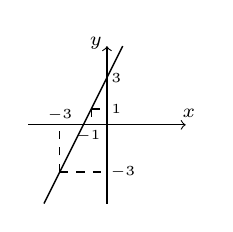
\begin{tikzpicture}[scale=0.2]
\tikzset {line01/.style={line width =0.5pt}}
\tikzset{line02/.style={line width =1pt}}
\tikzset{line03/.style={dashed,line width =0.5pt}}
%\filldraw [black] (0,0) circle (1pt);
\draw [->] (-5,0) -- (5,0);
\draw [->] (0,-5) -- (0,5);
\draw[line01] (-4,-5) -- (1,5);
\draw[line03] (-1,1) -- (-1,0);
\draw[line03] (-1,1) -- (0,1);
\draw[line03] (-3,-3) -- (-3,0);
\draw[line03] (-3,-3) -- (0,-3);
%\draw[line01] (0,-3) -- (-2,5);
\draw (0.6,3) node {\tiny $3$};
\draw (1,-3) node {\tiny $-3$};
\draw (-3,0.6) node {\tiny $-3$};
\draw (-1.2,-0.7) node {\tiny $-1$};
\draw (5.2,0.7) node {\scriptsize $x$};
\draw (0.6,1) node {\tiny $1$};
\draw (-0.7,5.2) node {\scriptsize $y$};
\end{tikzpicture}$$
34. Раз прямые параллельны, $k=-3.$ Подставим координаты точки $A:\ 4=(-3)\cdot1+b,\ b=7.$ Укажем три принадлежащие графику $y=-3x+7$ точки: $(-3;16),\ (0;7)$ и $(4;-5).$
$$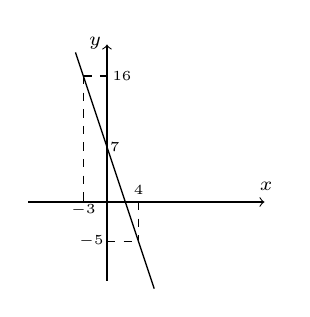
\begin{tikzpicture}[scale=0.1]
\tikzset {line01/.style={line width =0.5pt}}
\tikzset{line02/.style={line width =1pt}}
\tikzset{line03/.style={dashed,line width =0.5pt}}
%\filldraw [black] (0,0) circle (1pt);
\draw [->] (-10,0) -- (20,0);
\draw [->] (0,-10) -- (0,20);
\draw[line01] (-4,19) -- (6,-11);
\draw[line03] (-3,16) -- (0,16);
\draw[line03] (-3,16) -- (-3,0);
\draw[line03] (4,0) -- (4,-5);
\draw[line03] (0,-5) -- (4,-5);
%\draw[line03] (-1,1) -- (0,1);
%\draw[line03] (-1,0) -- (-1,1);
%\draw[line01] (0,-3) -- (-2,5);
%\draw (0.6,-4) node {\tiny $-4$};
%\draw (-1.6,-0.7) node {\tiny $-1$};
\draw (20.2,2) node {\scriptsize $x$};
\draw (-3,-1) node {\tiny $-3$};
\draw (4,1.5) node {\tiny $4$};
\draw (-2,-5) node {\tiny $-5$};
\draw (1,7) node {\tiny $7$};
\draw (1.9,16) node {\tiny $16$};
\draw (-1.5,20.2) node {\scriptsize $y$};
\end{tikzpicture}$$
35. Найдём точку пересечения прямых $y=x-7$ и $y=8x:\ x-7=8x,\ -7x=7,\ x=-1,\ y=8\cdot(-1)=-8.$ Найдём функцию $y=kx+b,$ график которой проходит через точки
$(9;-18)$ и $(-1;-8):\ \begin{cases} -18=9k+b,\\ -8=(-1)k+b.\end{cases}\Leftrightarrow \begin{cases} -10=10k,\\ -8=(-1)k+b.\end{cases}
\Leftrightarrow \begin{cases} k=-1,\\ b=-9.\end{cases}$ Построим прямую $y=-x-9$ по двум точкам $(-9;0)$ и $(0;-9).$
$$\begin{tikzpicture}[scale=0.1]
\tikzset {line01/.style={line width =0.5pt}}
\tikzset{line02/.style={line width =1pt}}
\tikzset{line03/.style={dashed,line width =0.5pt}}
%\filldraw [black] (0,0) circle (1pt);
\draw [->] (-20,0) -- (10,0);
\draw [->] (0,-20) -- (0,10);
\draw[line01] (-18,9) -- (6,-15);
%\draw[line03] (-3,16) -- (0,16);
%\draw[line03] (-3,16) -- (-3,0);
%\draw[line03] (4,0) -- (4,-5);
%\draw[line03] (0,-5) -- (4,-5);
%\draw[line03] (-1,1) -- (0,1);
%\draw[line03] (-1,0) -- (-1,1);
%\draw[line01] (0,-3) -- (-2,5);
%\draw (0.6,-4) node {\tiny $-4$};
%\draw (-1.6,-0.7) node {\tiny $-1$};
\draw (10.2,2) node {\scriptsize $x$};
%\draw (-3,-1) node {\tiny $-3$};
%\draw (4,1.5) node {\tiny $4$};
\draw (-10.1,-1) node {\tiny $-9$};
\draw (1.8,-9) node {\tiny $-9$};
%\draw (1,7) node {\tiny $7$};
%\draw (1.9,16) node {\tiny $16$};
\draw (-1.5,10.2) node {\scriptsize $y$};
\end{tikzpicture}$$
36. Найдём точку пересечения прямых $y=-3x$ и $y=x+12:\ -3x=x+12,\ -4x=12,\ x=-3,\ y=(-3)\cdot(-3)=9.$ Найдём функцию $y=kx+b,$ график которой проходит через точки
$(-6;12)$ и $(-3;9):\ \begin{cases} 12=-6k+b,\\ 9=-3k+b.\end{cases}\Leftrightarrow \begin{cases} 3=-3k,\\ 9=-3k+b.\end{cases}
\Leftrightarrow \begin{cases} k=-1,\\ b=6.\end{cases}$ Построим прямую $y=-x+6$ по двум точкам $(6;0)$ и $(0;6).$
$$\begin{tikzpicture}[scale=0.1]
\tikzset {line01/.style={line width =0.5pt}}
\tikzset{line02/.style={line width =1pt}}
\tikzset{line03/.style={dashed,line width =0.5pt}}
%\filldraw [black] (0,0) circle (1pt);
\draw [->] (-20,0) -- (10,0);
\draw [->] (0,-20) -- (0,10);
\draw[line01] (-5,11) -- (10,-4);
%\draw[line03] (-3,16) -- (0,16);
%\draw[line03] (-3,16) -- (-3,0);
%\draw[line03] (4,0) -- (4,-5);
%\draw[line03] (0,-5) -- (4,-5);
%\draw[line03] (-1,1) -- (0,1);
%\draw[line03] (-1,0) -- (-1,1);
%\draw[line01] (0,-3) -- (-2,5);
%\draw (0.6,-4) node {\tiny $-4$};
%\draw (-1.6,-0.7) node {\tiny $-1$};
\draw (10.2,2) node {\scriptsize $x$};
%\draw (-3,-1) node {\tiny $-3$};
%\draw (4,1.5) node {\tiny $4$};
\draw (6,-1) node {\tiny $6$};
\draw (1,6) node {\tiny $6$};
%\draw (1,7) node {\tiny $7$};
%\draw (1.9,16) node {\tiny $16$};
\draw (-1.5,10.2) node {\scriptsize $y$};
\end{tikzpicture}$$
37. Найдём точку пересечения прямых $y=2x+3$ и $y=8x+7:\ 2x+3=8x+7,\ -6x=4,\ x=-\cfrac{2}{3},\ y=2\cdot\left(-\cfrac{2}{3}\right)+3=\cfrac{5}{3}.$ Тогда необходимо построить график прямой $y=-6\cdot\left(-\cfrac{2}{3}\right)x+3\cdot\cfrac{5}{3}-9=4x-4.$ Построим его по двум точкам $(0;-4)$ и $(1;0).$
$$\begin{tikzpicture}[scale=0.2]
\tikzset {line01/.style={line width =0.5pt}}
\tikzset{line02/.style={line width =1pt}}
\tikzset{line03/.style={dashed,line width =0.5pt}}
%\filldraw [black] (0,0) circle (1pt);
\draw [->] (-10,0) -- (10,0);
\draw [->] (0,-10) -- (0,10);
\draw[line01] (3,8) -- (-1.5,-10);
%\draw[line03] (-1,1) -- (0,1);
%\draw[line03] (-1,0) -- (-1,1);
%\draw[line01] (0,-3) -- (-2,5);
%\draw (0.6,-4) node {\tiny $-4$};
%\draw (-1.6,-0.7) node {\tiny $-1$};
\draw (10.2,0.7) node {\scriptsize $x$};
\draw (-1,-4) node {\tiny $-4$};
\draw (1.1,-1) node {\tiny $1$};
\draw (0.7,10.2) node {\scriptsize $y$};
\end{tikzpicture}$$
38. Найдём точку пересечения прямых $y=2x-4$ и $y=8x-6:\ 2x-4=8x-6,\ -6x=-2,\ x=\cfrac{1}{3},\ y=2\cdot\left(\cfrac{1}{3}\right)-4=-\cfrac{10}{3}.$ Тогда необходимо построить график прямой $y=3\cdot\cfrac{1}{3}x-0,6\cdot \left(-\cfrac{10}{3}\right)=x+2.$ Построим его по двум точкам $(0;2)$ и $(-2;0).$
$$\begin{tikzpicture}[scale=0.2]
\tikzset {line01/.style={line width =0.5pt}}
\tikzset{line02/.style={line width =1pt}}
\tikzset{line03/.style={dashed,line width =0.5pt}}
%\filldraw [black] (0,0) circle (1pt);
\draw [->] (-10,0) -- (10,0);
\draw [->] (0,-10) -- (0,10);
\draw[line01] (6,8) -- (-8,-6);
%\draw[line03] (-1,1) -- (0,1);
%\draw[line03] (-1,0) -- (-1,1);
%\draw[line01] (0,-3) -- (-2,5);
%\draw (0.6,-4) node {\tiny $-4$};
%\draw (-1.6,-0.7) node {\tiny $-1$};
\draw (10.2,0.7) node {\scriptsize $x$};
\draw (1,2) node {\tiny $2$};
\draw (-2,-1) node {\tiny $-2$};
\draw (0.7,10.2) node {\scriptsize $y$};
\end{tikzpicture}$$
39. Раз график линейной функции $y=kx+b$ параллелен графику функции $y=-3x-7,$ её коэффициент $k=-3.$ Найдём точку пересечения прямых, заданных уравнениями $y=-2x+2$ и $y=3x-13:\ -2x+2=3x-13,\ -5x=-15,\ x=3,\ y=-2\cdot3+2=-4.$ Подставим координаты этой точки: $-4=(-3)\cdot3+b,\ b=5,$ то есть искомая функция имеет вид $y=-3x+5.$\\
40. Раз график линейной функции $y=kx+b$ параллелен графику функции $y=-2x+7,$ её коэффициент $k=-2.$ Найдём точку пересечения прямых, заданных уравнениями $y=2x+11$ и $y=-3x-9:\ 2x+11=-3x-9,\ 5x=-20,\ x=-4,\ y=2\cdot(-4)+11=3.$ Подставим координаты этой точки: $3=(-2)\cdot(-4)+b,\ b=-5,$ то есть искомая функция имеет вид $y=-2x-5.$\\
41. Найдём прямую $AB:\ \begin{cases} 3k+b=8,\\ 12k+b=5.\end{cases}\Leftrightarrow\begin{cases} -9k=3,\\ 12k+b=5.\end{cases}\Leftrightarrow
\begin{cases} k=-\cfrac{1}{3},\\ b=9.\end{cases}$ Найдём прямую $CD:\ \begin{cases} 4k+b=2,\\ 2k+b=-3.\end{cases}\Leftrightarrow\begin{cases} 2k=5,\\ 2k+b=-3.\end{cases}\Leftrightarrow
\begin{cases} k=\cfrac{5}{2},\\ b=-8.\end{cases}$ Найдём точку их пересечения: $-\cfrac{1}{3}x+9=\cfrac{5}{2}x-8,\ -\cfrac{17}{6}x=-17,\ x=6,\ y=-\cfrac{1}{3}\cdot6+9=7.$\\
42. Найдём прямую $AB:\ \begin{cases} 2k+b=4,\\ 4k+b=1.\end{cases}\Leftrightarrow\begin{cases} -2k=3,\\ 4k+b=1.\end{cases}\Leftrightarrow
\begin{cases} k=-\cfrac{3}{2},\\ b=7.\end{cases}$ Найдём прямую $CD:\ \begin{cases} 3k+b=-4,\\ 12k+b=2.\end{cases}\Leftrightarrow\begin{cases} -9k=-6,\\ 12k+b=2.\end{cases}\Leftrightarrow
\begin{cases} k=\cfrac{2}{3},\\ b=-6.\end{cases}$ Найдём точку их пересечения: $-\cfrac{3}{2}x+7=\cfrac{2}{3}x-6,\ -\cfrac{13}{6}x=-13,\ x=6,\ y=-\cfrac{3}{2}\cdot6+7=-2.$\\
43. Найдём прямую $AB:\ \begin{cases} 10k+b=-2,\\ 20k+b=3.\end{cases}\Leftrightarrow\begin{cases} -10k=-5,\\ 20k+b=3.\end{cases}
\Leftrightarrow\begin{cases} k=\cfrac{1}{2},\\ b=-7.\end{cases}$ Подставим в уравнение этой прямой координаты точки $C:\ \cfrac{1}{2}\cdot2016-7=1001.$ Полученное равенство верно, значит все три точки лежат на одной прямой.\\
44. Найдём прямую $AB:\ \begin{cases} 9k+b=-2,\\ 18k+b=1.\end{cases}\Leftrightarrow\begin{cases} -9k=-3,\\ 18k+b=1.\end{cases}
\Leftrightarrow\begin{cases} k=\cfrac{1}{3},\\ b=-5.\end{cases}$ Подставим в уравнение этой прямой координаты точки $C:\ \cfrac{1}{3}\cdot2016-5=667.$ Полученное равенство верно, значит все три точки лежат на одной прямой.\\
45. Найдём прямую $AB:\ \begin{cases} -\cfrac{1}{3}k+b=7,\\ 3k+b=-3.\end{cases}\Leftrightarrow\begin{cases} -\cfrac{10}{3}k=10,\\ 3k+b=-3.\end{cases}
\Leftrightarrow\begin{cases} k=-3,\\ b=6.\end{cases}$ Подставим в уравнение этой прямой координаты точки $C:\ p=(-3)\cdot\cfrac{p-1}{2}+6,\
2p=-3p+3+12,\ 5p=15,\ p=3.$ Эта прямая имеет уравнение $y=-3x+6.$\\
46. Найдём прямую $AB:\ \begin{cases} -\cfrac{1}{2}k+b=-5,\\ -4k+b=2.\end{cases}\Leftrightarrow\begin{cases} \cfrac{7}{2}k=-7,\\ -4k+b=2.\end{cases}
\Leftrightarrow\begin{cases} k=-2,\\ b=-6.\end{cases}$ Подставим в уравнение этой прямой координаты точки $C:\ p=(-2)\cdot\cfrac{p+2}{2}-6,\
p=-p-2-6,\ 2p=-8,\ p=-4.$ Эта прямая имеет уравнение $y=-2x-6.$\\
47. Найдём прямую, проходящую через данные точки: $\begin{cases} 4k+b=-5,\\ k^2+b=0.\end{cases}\Leftrightarrow
\begin{cases} 4k+b=-5,\\ k^2-4k-5=0.\end{cases}\Leftrightarrow\begin{cases} 4k+b=-5,\\ (k-5)(k+1)=0.\end{cases}\Leftrightarrow
\left[\begin{array}{l}\begin{cases} b=-25,\\ k=5.\end{cases}\\ \begin{cases} b=-1,\\ k=-1.\end{cases}\end{array}\right.$ Для нахождения точки пересечения необходимо решить систему уравнений: $\left[\begin{array}{l}\begin{cases} y=5x-25,\\ 5x-2y+17=0.\end{cases}\\ \begin{cases} y=-x-1,\\ 5x-2y+17=0.\end{cases}\end{array}\right.
\Leftrightarrow\left[\begin{array}{l}\begin{cases} y=5x-25,\\ 5x-10x+50+17=0.\end{cases}\\ \begin{cases} y=-x-1,\\ 5x+2x+2+17=0.\end{cases}\end{array}\right.
\Leftrightarrow\left[\begin{array}{l}\begin{cases} y=42,\\ x=\frac{67}{5}.\end{cases}\\ \begin{cases} y=\frac{12}{7},\\ x=-\frac{19}{7}.\end{cases}\end{array}\right.$ Первую прямую проведём через точки $(5;0)$ и $(0;-25),$ а вторую --- через точки $(-1;0)$ и $(0;-1).$
$$\begin{array}{lr}
\begin{tikzpicture}[scale=0.2]
\tikzset {line01/.style={line width =0.5pt}}
\tikzset{line02/.style={line width =1pt}}
\tikzset{line03/.style={dashed,line width =0.5pt}}
%\filldraw [black] (0,0) circle (1pt);
\draw [->] (-5,0) -- (10,0);
\draw [->] (0,-30) -- (0,10);
\draw[line01] (6,5) -- (-1,-30);
%\draw[line03] (-1,1) -- (0,1);
%\draw[line03] (-1,0) -- (-1,1);
%\draw[line01] (0,-3) -- (-2,5);
%\draw (0.6,-4) node {\tiny $-4$};
%\draw (-1.6,-0.7) node {\tiny $-1$};
\draw (10.2,0.7) node {\scriptsize $x$};
\draw (1,-25) node {\tiny $-25$};
\draw (5.3,-1) node {\tiny $5$};
\draw (0.7,10.2) node {\scriptsize $y$};
\end{tikzpicture}&
\begin{tikzpicture}[scale=0.2]
\tikzset {line01/.style={line width =0.5pt}}
\tikzset{line02/.style={line width =1pt}}
\tikzset{line03/.style={dashed,line width =0.5pt}}
%\filldraw [black] (0,0) circle (1pt);
\draw [->] (-10,0) -- (10,0);
\draw [->] (0,-10) -- (0,10);
\draw[line01] (6,-7) -- (-8,7);
%\draw[line03] (-1,1) -- (0,1);
%\draw[line03] (-1,0) -- (-1,1);
%\draw[line01] (0,-3) -- (-2,5);
%\draw (0.6,-4) node {\tiny $-4$};
%\draw (-1.6,-0.7) node {\tiny $-1$};
\draw (10.2,0.7) node {\scriptsize $x$};
\draw (1,-1) node {\tiny $-1$};
\draw (-1,1) node {\tiny $-1$};
\draw (0.7,10.2) node {\scriptsize $y$};
\end{tikzpicture}\end{array}$$
48. Найдём точку пересечения прямых $y=\cfrac{x}{3}-8,5$ и $y=-6x+20:\ \cfrac{x}{3}-8,5=-6x+20,\ \cfrac{19}{3}x=28,5,\ x=\cfrac{9}{2},\ y=-7.$ Подставим её координаты в уравнение прямой $y=(2m+1)x+1-4m:\ -7=(2m+1)\cdot\cfrac{9}{2}+1-4m,\ -14=18m+9+2-8m,\ -10m=25,\ m=-\cfrac{5}{2}.$\\
49. Найдём точку пересечения прямых $y=\cfrac{x}{3}-6,5$ и $y=-4x+26:\ \cfrac{x}{3}-6,5=-4x+26,\ \cfrac{13}{3}x=32,5,\ x=\cfrac{15}{2},\ y=-4.$ Подставим её координаты в уравнение прямой $y=(2t-1)x+9,5-5t:\ -4=(2t-1)\cdot\cfrac{15}{2}+9,5-5t,\ -8=30t-15+19-10t,\ -20t=12,\ t=-\cfrac{3}{5}.$\\
50. Найдём точку пересечения прямых, заданных уравнениями $y=2x-5$ и $y=-x+4:\ 2x-5=-x+4,\ 3x=9,\ x=3,\ y=-3+4=1.$ Раз прямая $y=kx+b$ параллельна прямой $y=-\cfrac{1}{2}x+11,$ её коэффициент $k=-\cfrac{1}{2}.$ Подставим в её уравнение координаты найденной точки: $1=-\cfrac{1}{2}\cdot3+b,\ b=\cfrac{5}{2}.$
Проведём прямую через две точки $\left(0;\cfrac{5}{2}\right)$ и $(5;0).$
$$\begin{tikzpicture}[scale=0.2]
\tikzset {line01/.style={line width =0.5pt}}
\tikzset{line02/.style={line width =1pt}}
\tikzset{line03/.style={dashed,line width =0.5pt}}
%\filldraw [black] (0,0) circle (1pt);
\draw [->] (-10,0) -- (10,0);
\draw [->] (0,-10) -- (0,10);
\draw[line01] (7,-1) -- (-7,6);
%\draw[line03] (-1,1) -- (0,1);
%\draw[line03] (-1,0) -- (-1,1);
%\draw[line01] (0,-3) -- (-2,5);
%\draw (0.6,-4) node {\tiny $-4$};
%\draw (-1.6,-0.7) node {\tiny $-1$};
\draw (10.2,0.7) node {\scriptsize $x$};
\draw (1,3) node {\tiny $\frac{5}{2}$};
\draw (5,1) node {\tiny $5$};
\draw (5,-4) node {\scriptsize $y=-\frac{1}{2}x+\frac{5}{2}$};
\draw (0.7,10.2) node {\scriptsize $y$};
\end{tikzpicture}$$
51. Найдём точку пересечения прямых, заданных уравнениями $y=-2x+4$ и $y=\cfrac{1}{2}x+1:\ -2x+4=\cfrac{1}{2}x+1,\ -\cfrac{5}{2}x=-3,\ x=\cfrac{6}{5},\ y=-\cfrac{12}{5}+4=\cfrac{8}{5}.$ Раз прямая $y=kx+b$ параллельна прямой $y=-\cfrac{1}{3}x-21,$ её коэффициент $k=-\cfrac{1}{3}.$ Подставим в её уравнение координаты найденной точки: $\cfrac{8}{5}=-\cfrac{1}{3}\cdot\cfrac{6}{5}+b,\ b=2.$
Проведём прямую через две точки $\left(0;2\right)$ и $(6;0).$
$$\begin{tikzpicture}[scale=0.2]
\tikzset {line01/.style={line width =0.5pt}}
\tikzset{line02/.style={line width =1pt}}
\tikzset{line03/.style={dashed,line width =0.5pt}}
%\filldraw [black] (0,0) circle (1pt);
\draw [->] (-10,0) -- (10,0);
\draw [->] (0,-10) -- (0,10);
\draw[line01] (9,-1) -- (-6,4);
%\draw[line03] (-1,1) -- (0,1);
%\draw[line03] (-1,0) -- (-1,1);
%\draw[line01] (0,-3) -- (-2,5);
%\draw (0.6,-4) node {\tiny $-4$};
%\draw (-1.6,-0.7) node {\tiny $-1$};
\draw (10.2,0.7) node {\scriptsize $x$};
\draw (0.5,2.3) node {\tiny $2$};
\draw (6,-0.5) node {\tiny $6$};
\draw (6,-4) node {\scriptsize $y=-\frac{1}{3}x+2$};
\draw (0.7,10.2) node {\scriptsize $y$};
\end{tikzpicture}$$
52. $y=\cfrac{x^2}{x-1}-\cfrac{1}{x-1}=\cfrac{x^2-1}{x-1}=\cfrac{(x-1)(x+1)}{x-1}=x+1$ при условии $x\neq1.$ Проведём прямую через точки $(-1;0)$ и $(0;1),$ не забыв выколоть точку $(1;2).$
$$\begin{tikzpicture}[scale=0.6]
\tikzset {line01/.style={line width =0.5pt}}
\tikzset{line02/.style={line width =1pt}}
\tikzset{line03/.style={dashed,line width =0.5pt}}
\draw [->] (-3,0) -- (3,0);
\draw [->] (0,-3) -- (0,3);
\draw[line01] (-1.9,-0.9) -- (1.9,2.9);
\draw[line03] (0,2) -- (1,2);
\draw[line03] (1,0) -- (1,2);
\draw (1,2) circle (3pt);
\draw (-0.2,2) node {\tiny $2$};
\draw (-0.2,1) node {\tiny $1$};
\draw (1,-0.2) node {\tiny $1$};
\draw (-1,-0.2) node {\tiny $-1$};
\draw (3,0.25) node {\scriptsize $x$};
\draw (0.25,3) node {\scriptsize $y$};
\end{tikzpicture}$$
53. а) Найдём эту прямую: $\begin{cases} -2a+b=-1,\\ a+b=5.\end{cases}\Leftrightarrow\begin{cases} -3a=-6,\\ a+b=5.\end{cases}\Leftrightarrow
\begin{cases} a=2,\\ b=3.\end{cases}$\\
б) Эта прямая должна проходить только через точки II и IV четверти или оси координат, значит она проходит через начало координат и $a\leqslant0,\ b=0.$\\
54. $(y-2)(x-y)=0\Leftrightarrow\left[\begin{array}{l} y-2=0,\\ x-y=0.\end{array}\right.\Leftrightarrow\left[\begin{array}{l} y=2,\\ y=x.\end{array}\right.$
$$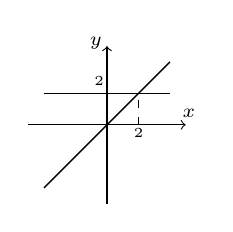
\begin{tikzpicture}[scale=0.2]
\tikzset {line01/.style={line width =0.5pt}}
\tikzset{line02/.style={line width =1pt}}
\tikzset{line03/.style={dashed,line width =0.5pt}}
%\filldraw [black] (0,0) circle (1pt);
\draw [->] (-5,0) -- (5,0);
\draw [->] (0,-5) -- (0,5);
\draw[line01] (-4,2) -- (4,2);
\draw[line01] (-4,-4) -- (4,4);
\draw[line03] (2,0) -- (2,2);
\draw (2,-0.5) node {\tiny $2$};
\draw (-0.5,2.8) node {\tiny $2$};
\draw (5.2,0.7) node {\scriptsize $x$};
\draw (-0.7,5.2) node {\scriptsize $y$};
\end{tikzpicture}$$
55. $|y|=|x+1|\Leftrightarrow\left[\begin{array}{l} y=x+1,\\ y=-x-1.\end{array}\right.$
$$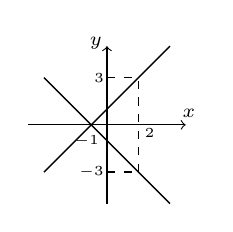
\begin{tikzpicture}[scale=0.2]
\tikzset {line01/.style={line width =0.5pt}}
\tikzset{line02/.style={line width =1pt}}
\tikzset{line03/.style={dashed,line width =0.5pt}}
%\filldraw [black] (0,0) circle (1pt);
\draw [->] (-5,0) -- (5,0);
\draw [->] (0,-5) -- (0,5);
\draw[line01] (-4,3) -- (4,-5);
\draw[line01] (-4,-3) -- (4,5);
\draw[line03] (2,-3) -- (2,3);
\draw[line03] (0,3) -- (2,3);
\draw[line03] (0,-3) -- (2,-3);
\draw (2.7,-0.5) node {\tiny $2$};
\draw (-1.3,-1) node {\tiny $-1$};
\draw (-0.5,3) node {\tiny $3$};
\draw (-1,-3) node {\tiny $-3$};
\draw (5.2,0.7) node {\scriptsize $x$};
\draw (-0.7,5.2) node {\scriptsize $y$};
\end{tikzpicture}$$
\newpage
\noindent56. Возможны три случая: точки $A$ и $B$ являются противоположными вершинами квадрата, $A$ и $B$ являются соседними вершинами и две других вершины над прямой $AB$ и $A$ и $B$ являются соседними вершинами и две других вершины под прямой $AB.$ Во всех случаях две оставшихся вершины достраиваются <<по клеточкам>>.
\begin{figure}[h]
\begin{center}
\begin{minipage}[h]{0.2\linewidth}
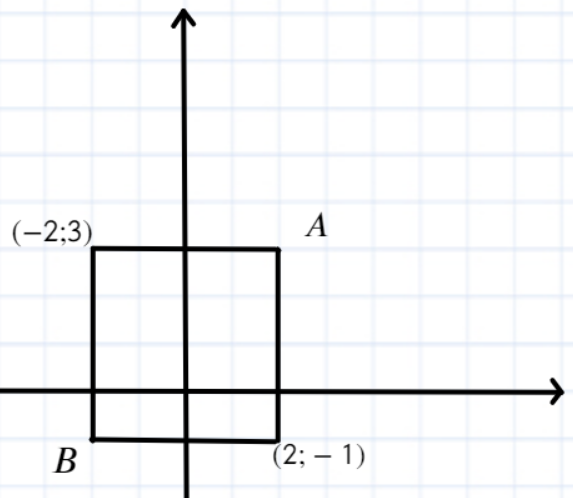
\includegraphics[width=1\linewidth]{kv1.png}
 %% метка рисунка для ссылки на него
\end{minipage}
\hfill
\begin{minipage}[h]{0.4\linewidth}
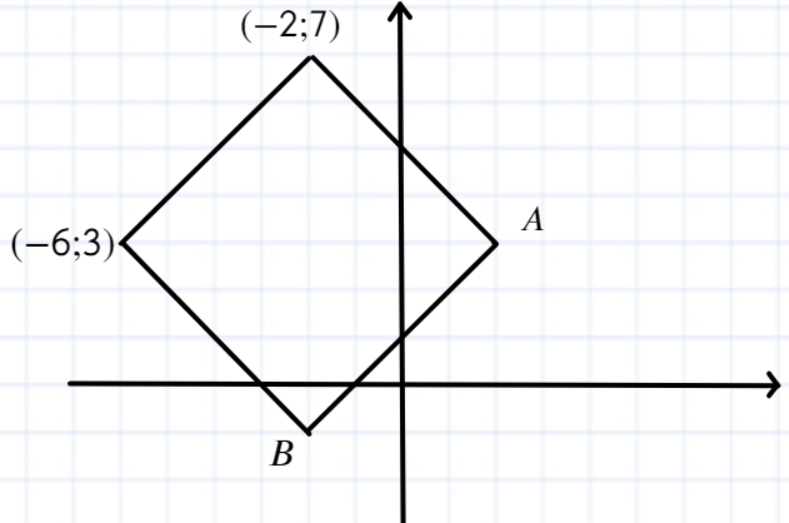
\includegraphics[width=1\linewidth]{kv2.png}
\end{minipage}
\hfill
\begin{minipage}[h]{0.2\linewidth}
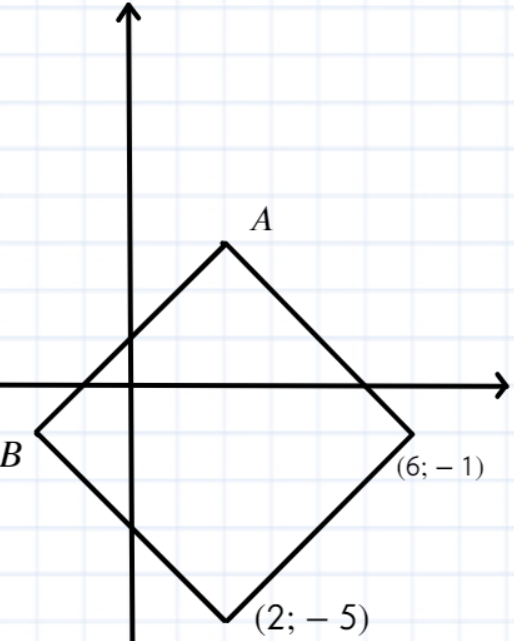
\includegraphics[width=1\linewidth]{kv3.png}
 %% метка рисунка для ссылки на него
\end{minipage}
\hfill
\end{center}
\end{figure}\\
57. Найдём точку, в которой прямая $y=-0,5x+4$ пересекает ось $Ox$ (в ней $y=0):\ 0=-0,5x+4,\ x=8$ и ось $Oy$ (в ней $x=0):\ y=-0,5\cdot0+4=4.$ Если $BA$ является медианой, точка $A$ лежит посередине между $O$ и $C,$ а значит точка $C$ имеет координаты $(0;8).$ Проведём прямую через неё и точку $B(8;0):\
\begin{cases} 8=0+b,\\ 0=8k+b.\end{cases}\Rightarrow y=-x+8.$
$$\begin{tikzpicture}[scale=0.2]
\tikzset {line01/.style={line width =0.5pt}}
\tikzset{line02/.style={line width =1pt}}
\tikzset{line03/.style={dashed,line width =0.5pt}}
%\filldraw [black] (0,0) circle (1pt);
\draw [->] (-10,0) -- (10,0);
\draw [->] (0,-10) -- (0,10);
\draw[line01] (9,-1) -- (-1,9);
%\draw[line03] (-1,1) -- (0,1);
%\draw[line03] (-1,0) -- (-1,1);
%\draw[line01] (0,-3) -- (-2,5);
%\draw (0.6,-4) node {\tiny $-4$};
%\draw (-1.6,-0.7) node {\tiny $-1$};
\draw (10.2,0.7) node {\scriptsize $x$};
\draw (0.5,8) node {\tiny $8$};
\draw (8,0.5) node {\tiny $8$};
\draw (0.7,10.2) node {\scriptsize $y$};
\end{tikzpicture}$$
58. $y=(x^2-4)\left(\cfrac{1}{x-2}-\cfrac{1}{x+2}\right)-x=(x-2)(x+2)\cdot\cfrac{x+2-x+2}{(x-2)(x+2)}-x=4-x,$ при этом $x\neq\pm2.$ Проведём прямую через точки $(0;4)$ и $(4;0),$ не забыв выколоть точки $(-2;6)$ и $(2;2).$
$$\begin{tikzpicture}[scale=0.2]
\tikzset {line01/.style={line width =0.5pt}}
\tikzset{line02/.style={line width =1pt}}
\tikzset{line03/.style={dashed,line width =0.5pt}}
%\filldraw [black] (0,0) circle (1pt);
\draw [->] (-10,0) -- (10,0);
\draw [->] (0,-10) -- (0,10);
\draw[line01] (-6,10) -- (8,-4);
\draw (10.2,0.7) node {\scriptsize $x$};
\draw (-2.5,-0.7) node {\scriptsize $-2$};
\draw (2,-0.7) node {\scriptsize $2$};
\draw (-0.7,2) node {\scriptsize $2$};
\draw (0.7,6) node {\scriptsize $6$};
%\draw (-5.5,-2) node {\scriptsize $-6$};
\draw[line03] (-2,0) -- (-2,6);
\draw[line03] (0,6) -- (-2,6);
\draw[line03] (2,0) -- (2,2);
\draw[line03] (0,2) -- (2,2);
\draw (0.7,10.2) node {\scriptsize $y$};
\draw (2,2) circle (10pt);
\draw (-2,6) circle (10pt);
\end{tikzpicture}$$
59. $y=\cfrac{|x|}{x}\left(-\cfrac{1}{2}x+2\right)=\left[\begin{array}{l}\cfrac{1}{2}x-2, x<0,\\ -\cfrac{1}{2}x+2, x>0.\end{array}\right.$
Проведём прямые через точки $(-4;-4)$ и $(0;-2)$ и $(0;2)$ и $(4;0),$ не забыв выколоть точки $(0;-2)$ и $(0;2).$
$$\begin{tikzpicture}[scale=0.2]
\tikzset {line01/.style={line width =0.5pt}}
\tikzset{line02/.style={line width =1pt}}
\tikzset{line03/.style={dashed,line width =0.5pt}}
%\filldraw [black] (0,0) circle (1pt);
\draw [->] (-10,0) -- (10,0);
\draw [->] (0,-10) -- (0,10);
\draw[line01] (0,2) -- (8,-2);
\draw[line01] (0,-2) -- (-8,-6);
\draw (10.2,0.7) node {\scriptsize $x$};
\draw (4,0.7) node {\scriptsize $4$};
\draw (-4,0.7) node {\scriptsize $-4$};
\draw (-1,2) node {\scriptsize $2$};
\draw (1.4,-2) node {\scriptsize $-2$};
\draw (1.2,-4) node {\scriptsize $-4$};
\draw (0.7,10.2) node {\scriptsize $y$};
\draw (0,2) circle (10pt);
\draw (0,-2) circle (10pt);
\draw[line03] (-4,0) -- (-4,-4);
\draw[line03] (0,-4) -- (-4,-4);
\end{tikzpicture}$$
60. $\cfrac{(y^2-4)(y+2x-1)}{x-1}=0\Leftrightarrow\cfrac{(y-2)(y+2)(y-(1-2x))}{x-1}=0\Leftrightarrow\begin{cases}
\left[\begin{array}{l} y=2,\\ y=-2, \\ y=1-2x.\end{array}\right.\\ x\neq1.\end{cases}$
$$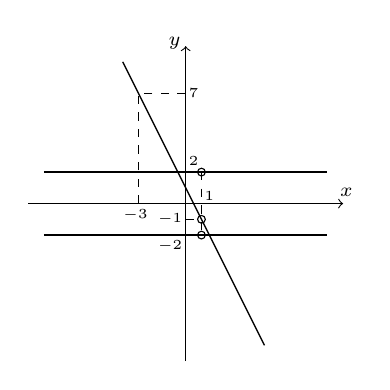
\begin{tikzpicture}[scale=0.2]
\tikzset {line01/.style={line width =0.5pt}}
\tikzset{line02/.style={line width =1pt}}
\tikzset{line03/.style={dashed,line width =0.5pt}}
%\filldraw [black] (0,0) circle (1pt);
\draw [->] (-10,0) -- (10,0);
\draw [->] (0,-10) -- (0,10);
\draw[line01] (-9,2) -- (9,2);
\draw[line01] (-9,-2) -- (9,-2);
\draw[line01] (5,-9) -- (-4,9);
\draw[line03] (1,2) -- (1,-2);
\draw[line03] (0,-1) -- (1,-1);
\draw[line03] (-3,0) -- (-3,7);
\draw[line03] (0,7) -- (-3,7);
\draw (1.5,0.5) node {\tiny $1$};
\draw (-3.2,-0.7) node {\tiny $-3$};
\draw (0.5,7) node {\tiny $7$};
\draw (0.5,2.7) node {\tiny $2$};
\draw (-1,-2.7) node {\tiny $-2$};
\draw (-1,-1) node {\tiny $-1$};
\draw (10.2,0.7) node {\scriptsize $x$};
\draw (-0.7,10.2) node {\scriptsize $y$};
\draw (1,2) circle (7pt);
\draw (1,-2) circle (7pt);
\draw (1,-1) circle (7pt);
\end{tikzpicture}$$
61. Приведём пример одной из возможных кусочно-линейных функций и нарисуем её график:
$$y=\begin{cases} 0,\ 0<x\leqslant\cfrac{1}{3},\\
3x-1,\ \cfrac{1}{3}<x\leqslant\cfrac{2}{3},\\
1,\ \cfrac{2}{3}<x<1.\end{cases}$$
$$\begin{tikzpicture}[scale=0.4]
\tikzset {line01/.style={line width =1pt}}
\tikzset{line02/.style={line width =1pt}}
\tikzset{line03/.style={dashed,line width =0.5pt}}
%\filldraw [black] (0,0) circle (1pt);
\draw [->] (-6,0) -- (10,0);
\draw [->] (0,-6) -- (0,10);
\draw[line01] (0,0) -- (1,0);
\draw[line01] (1,0) -- (2,3);
\draw[line01] (2,3) -- (3,3);
\draw (3,-0.5) node {\tiny $1$};
\draw (-0.5,3) node {\tiny $1$};
\draw (0,0) circle (10pt);
\draw (3,3) circle (10pt);
\draw (10.2,0.7) node {\scriptsize $x$};
\draw (-0.7,10.2) node {\scriptsize $y$};
\draw[line03] (0,3) -- (3,3);
\draw[line03] (3,0) -- (3,3);
\end{tikzpicture}
$$
62. Подставим в уравнение данной функции точку $(0;0):\ 0=\cfrac{5a}{a-5}\cdot(0-1)+\cfrac{a^2}{a-5},\ 0=\cfrac{a^2-5a}{a-5}=\cfrac{a(a-5)}{a-5}=0,\ a=0.$\\
63. У точек на оси абсцисс координата $y=0,$ подставим значения $x$ и $y$ в уравнение графика функции:
$0=\cfrac{-\cfrac{4}{3}-b}{3\cdot\left(-\cfrac{4}{3}\right)+1}+b\cdot\left(-\cfrac{4}{3}\right),\ \cfrac{4}{3}+b-4b=0,\ b=\cfrac{4}{9}.$\\
64. $y=(2-0,5x): (-0,125)=4x-16.$ У этих функций одинаковый коэффициент $k,$ значит они не пересекаются. Оси они пересекают в точках $(0;-16),\ (4;0),\ (0;-1),\ \left(\cfrac{1}{4};0\right).$
$$\begin{tikzpicture}[scale=0.2]
\tikzset {line01/.style={line width =0.5pt}}
\tikzset{line02/.style={line width =1pt}}
\tikzset{line03/.style={dashed,line width =0.5pt}}
%\filldraw [black] (0,0) circle (1pt);
\draw [->] (-5,0) -- (10,0);
\draw [->] (0,-20) -- (0,11);
\draw[line01] (-1,-20) -- (6,8);
\draw[line01] (-1,-5) -- (3,11);
%\draw[line03] (-1,1) -- (0,1);
%\draw[line03] (-1,0) -- (-1,1);
%\draw[line01] (0,-3) -- (-2,5);
%\draw (0.6,-4) node {\tiny $-4$};
%\draw (-1.6,-0.7) node {\tiny $-1$};
\draw (10.2,0.7) node {\scriptsize $x$};
\draw (4.3,-1) node {\tiny $4$};
\draw (0.5,-1) node {\tiny $\frac{1}{4}$};
\draw (-1,-1) node {\tiny $-1$};
\draw (-1.5,-16) node {\tiny $-16$};
\draw (0.7,11.2) node {\scriptsize $y$};
\end{tikzpicture}$$
65. Найдём точку пересечения прямых $y=\cfrac{1}{3}x-2$ и $y=6-x:\ \cfrac{1}{3}x-2=6-x,\ \cfrac{4}{3}x=8,\ x=6,\ y=6-x=0.$ Прямая $y=-4x-3$ пересекает ось $Oy$ в точке с абсциссой $x=0$ и ординатой $y=0-3=-3.$ Найдём прямую, проходящую через полученные точки: $\begin{cases} 6k+b=0,\\ 0+b=-3.\end{cases}\Leftrightarrow
\begin{cases} k=\cfrac{1}{2},\\ b=-3.\end{cases}$ Проведём прямую через две точки $(0;-3)$ и $(6;0).$
$$\begin{tikzpicture}[scale=0.2]
\tikzset {line01/.style={line width =0.5pt}}
\tikzset{line02/.style={line width =1pt}}
\tikzset{line03/.style={dashed,line width =0.5pt}}
%\filldraw [black] (0,0) circle (1pt);
\draw [->] (-6.5,0) -- (10,0);
\draw [->] (0,-10) -- (0,10);
\draw[line01] (8,1) -- (-6,-6);
%\draw[line03] (-1,1) -- (0,1);
%\draw[line03] (-1,0) -- (-1,1);
%\draw[line01] (0,-3) -- (-2,5);
%\draw (0.6,-4) node {\tiny $-4$};
%\draw (-1.6,-0.7) node {\tiny $-1$};
\draw (10.2,0.7) node {\scriptsize $x$};
\draw (1,-3) node {\tiny $-3$};
\draw (6,-0.5) node {\tiny $6$};
\draw (0.7,10.2) node {\scriptsize $y$};
\end{tikzpicture}$$
66. а) Проведём прямую через две точки $(-1;1)$ и $(0;3).$
$$\begin{tikzpicture}[scale=0.2]
\tikzset {line01/.style={line width =0.5pt}}
\tikzset{line02/.style={line width =1pt}}
\tikzset{line03/.style={dashed,line width =0.5pt}}
%\filldraw [black] (0,0) circle (1pt);
\draw [->] (-6.5,0) -- (10,0);
\draw [->] (0,-10) -- (0,10);
\draw[line01] (-4,-5) -- (3,9);
\draw[line03] (-1,1) -- (0,1);
\draw[line03] (-1,0) -- (-1,1);
%\draw[line01] (0,-3) -- (-2,5);
%\draw (0.6,-4) node {\tiny $-4$};
%\draw (-1.6,-0.7) node {\tiny $-1$};
\draw (10.2,0.7) node {\scriptsize $x$};
\draw (0.5,3) node {\tiny $3$};
\draw (0.5,1) node {\tiny $1$};
\draw (-1.5,-1) node {\tiny $-1$};
\draw (0.7,10.2) node {\scriptsize $y$};
\end{tikzpicture}$$
б) Подставим координаты точки $A$ в уравнение прямой: $1=k\cdot(-1)+3,\ k=2.$\\
в) Ось абсцисс эта прямая пересекает в точке $\left(-\cfrac{3}{2};0\right)$ и образует прямоугольный треугольник с катетами $\cfrac{3}{2}$ и $3.$ Его площадь равна $\cfrac{1}{2}\cdot\cfrac{3}{2}\cdot3=\cfrac{9}{4}.$\\
г) Так как угловые коэффициенты у этих прямых разные, они пересекаются.\\
67. а) Это прямоугольник, ограниченный прямыми $x=3,\ x=9,\ y=-3,\ y=6.$
$$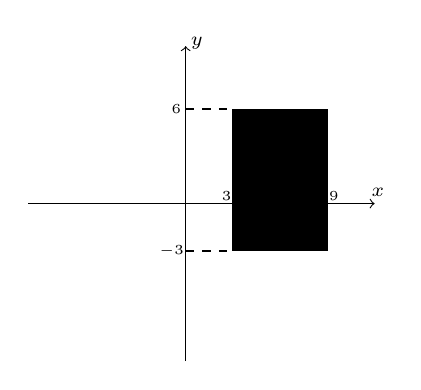
\begin{tikzpicture}[scale=0.2]
\tikzset {line01/.style={line width =0.5pt}}
\tikzset{line02/.style={line width =1pt}}
\tikzset{line03/.style={dashed,line width =0.5pt}}
%\filldraw [black] (0,0) circle (1pt);
\draw [->] (-10,0) -- (12,0);
\draw [->] (0,-10) -- (0,10);
\filldraw [draw=black] (3,-3) rectangle (9,6);
\draw[line03] (0,-3) -- (3,-3);
\draw[line03] (0,6) -- (3,6);
%\draw[line03] (-1,0) -- (-1,1);
%\draw[line01] (0,-3) -- (-2,5);
%\draw (0.6,-4) node {\tiny $-4$};
%\draw (-1.6,-0.7) node {\tiny $-1$};
\draw (12.2,0.7) node {\scriptsize $x$};
\draw (2.6,0.5) node {\tiny $3$};
\draw (-0.9,-3) node {\tiny $-3$};
\draw (-0.6,6) node {\tiny $6$};
\draw (9.4,0.5) node {\tiny $9$};
%\draw (-2.2,1) node {\tiny $-\frac{3}{2}$};
\draw (0.7,10.2) node {\scriptsize $y$};
\end{tikzpicture}$$
б) Горизонтальная сторона этого прямоугольника равна $a+6-a=6,$ а вертикальная --- $2a-(-a)=3a.$ Он является квадратом при $3a=6,\ a=2.$\\
68. Построим каждую из прямых по двум точкам, отмеченным на рисунке (они найдены как точки пересечения данных прямых).
$$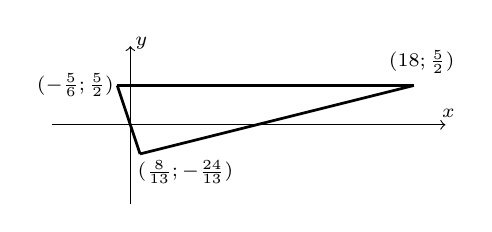
\begin{tikzpicture}[scale=0.2]
\tikzset {line01/.style={line width =0.5pt}}
\tikzset{line02/.style={line width =1pt}}
\tikzset{line03/.style={dashed,line width =0.5pt}}
%\filldraw [black] (0,0) circle (1pt);
\draw [->] (-5,0) -- (20,0);
\draw [->] (0,-5) -- (0,5);
\draw[line02] (18,2.5) -- (-0.833,2.5);
\draw[line02] (18,2.5) -- (0.615,-1.846);
\draw[line02] (0.615,-1.846) -- (-0.833,2.5);
\draw (20.2,0.7) node {\scriptsize $x$};
\draw (-3.5,2.5) node {\scriptsize $(-\frac{5}{6};\frac{5}{2})$};
\draw (3.5,-3) node {\scriptsize $(\frac{8}{13};-\frac{24}{13})$};
\draw (18.5,4) node {\scriptsize $(18;\frac{5}{2})$};
\draw (0.7,5.2) node {\scriptsize $y$};
\end{tikzpicture}$$
69. Найдём прямую, проходящую через точки $M(2;-5)$ и $N(0;-2): \begin{cases} 2k+b=-5,\\ b=-2.\end{cases}\Leftrightarrow\begin{cases} k=-\cfrac{3}{2},\\ b=-2.\end{cases}$ Приведём уравнение этой прямой к искомому виду: $y=-\cfrac{3}{2}x-2,\ 2y=-3x-4,\ 3x+2y=-4.$\\
70. Построим квадрат с вершинами $(-1;5),\ (-1;1),\ (3;5)$ и $(3;1).$ Тогда прямая $y=x+2$ является его диагональю и вершине $A(3;1)$ относительно диагонали симметрична вершина $(-1;5).$\\
71. а) $\cfrac{x}{x^2+2x+4}+\cfrac{x^2+8}{x^3-8}-\cfrac{1}{x-2}=\cfrac{x}{x^2+2x+4}+\cfrac{x^2+8}{(x-2)(x^2+2x+4)}-\cfrac{1}{x-2}=$\\$
\cfrac{x^2-2x+x^2+8-x^2-2x-4}{(x-2)(x^2+2x+4)}=\cfrac{x^2-4x+4}{(x-2)(x^2+2x+4)}=\cfrac{(x-2)^2}{(x-2)(x^2+2x+4)}=\cfrac{x-2}{x^2+2x+4}.$\\
$\cfrac{x^2}{x^2-4}-\cfrac{2}{2-x}=\cfrac{x^2}{(x-2)(x+2)}+\cfrac{2}{x-2}=\cfrac{x^2+2x+4}{(x-2)(x+2)}.$\\
$\cfrac{x-2}{x^2+2x+4}\cdot\cfrac{x^2+2x+4}{(x-2)(x+2)}=\cfrac{1}{x+2}.$\\
б) $y=\cfrac{1}{f(x)}=x+2,$ при этом нельзя брать $x=\pm2,$ так как эти значения обнуляли знаменатель.
$$\begin{tikzpicture}[scale=0.2]
\tikzset {line01/.style={line width =0.5pt}}
\tikzset{line02/.style={line width =1pt}}
\tikzset{line03/.style={dashed,line width =0.5pt}}
%\filldraw [black] (0,0) circle (1pt);
\draw [->] (-10,0) -- (10,0);
\draw [->] (0,-10) -- (0,10);
\draw[line01] (-6,-4) -- (8,10);
\draw (10.2,0.7) node {\scriptsize $x$};
\draw (-1.9,-1.5) node {\scriptsize $-2$};
\draw (2,-0.7) node {\scriptsize $2$};
\draw (-0.7,4) node {\scriptsize $4$};
%\draw (0.7,6) node {\scriptsize $6$};
%\draw (-5.5,-2) node {\scriptsize $-6$};
\draw[line03] (2,0) -- (2,4);
\draw[line03] (0,4) -- (2,4);
\draw (0.7,10.2) node {\scriptsize $y$};
\draw (2,4) circle (10pt);
\draw (-2,0) circle (10pt);
\end{tikzpicture}$$
72. а) Найдём прямую $AB:\ \begin{cases} b=-7,\\ 3k+b=2.\end{cases}\Leftrightarrow\begin{cases} b=-7,\\ k=3.\end{cases}\Rightarrow y=3x-7.$
Найдём прямую $CD:\ \begin{cases} k+b=1,\\ -30k+b=63.\end{cases}\Leftrightarrow\begin{cases} 31k=-62,\\ -30k+b=63.\end{cases}
\Leftrightarrow\begin{cases} k=-2,\\ b=3.\end{cases}\Rightarrow y=-2x+3.$\\
б) Найдём точку пересечения прямых $AB$ и $CD: 3x-7=-2x+3,\ 5x=10,\ x=2,\ y=3\cdot2-7=-1.$ Найдём прямую $BC:\ \begin{cases} 3k+b=2,\\ k+b=1.\end{cases}\Leftrightarrow\begin{cases} 2k=1,\\ k+b=1.\end{cases}\Leftrightarrow\begin{cases} k=\cfrac{1}{2},\\ b=\cfrac{1}{2}.\end{cases}\Rightarrow y=\cfrac{1}{2}x+\cfrac{1}{2}.$ Точка этой прямой, лежащая на оси абсцисс, имеет ординату $y=0,$ а значит $\cfrac{1}{2}x+\cfrac{1}{2}=0,\ x=-1.$ Таким образом, необходимо найти уравнение прямой, проходящей через точки $(2;-1)$ и $(-1;0): \ \begin{cases} 2k+b=-1,\\ -k+b=0.\end{cases}\Leftrightarrow\begin{cases} 3k=-1,\\ -k+b=0.\end{cases}\Leftrightarrow\begin{cases} k=-\cfrac{1}{3},\\ b=-\cfrac{1}{3}.\end{cases}\Rightarrow y=-\cfrac{1}{3}x-\cfrac{1}{3}.$\\
73. а) Найдём прямую $AC:\ \begin{cases} b=4,\\ -3k+b=-2.\end{cases}\Leftrightarrow\begin{cases} b=4,\\ k=2.\end{cases}\Rightarrow y=2x+4.$
Найдём прямую $BD:\ \begin{cases} k+b=-4,\\ -20k+b=59.\end{cases}\Leftrightarrow\begin{cases} 21k=-63,\\ -20k+b=59.\end{cases}
\Leftrightarrow\begin{cases} k=-3,\\ b=-1.\end{cases}\Rightarrow y=-3x-1.$\\
б) Найдём точку пересечения прямых $AC$ и $BD: 2x+4=-3x-1,\ 5x=-5,\ x=-1,\ y=2\cdot(-1)+4=2.$ Найдём прямую $BC:\ \begin{cases} k+b=-4,\\ -3k+b=-2.\end{cases}\Leftrightarrow\begin{cases} 4k=-2,\\ -3k+b=-2.\end{cases}\Leftrightarrow\begin{cases} k=-\cfrac{1}{2},\\ b=-\cfrac{7}{2}.\end{cases}\Rightarrow y=-\cfrac{1}{2}x-\cfrac{7}{2}.$ Точка этой прямой, лежащая на оси абсцисс, имеет ординату $y=0,$ а значит $-\cfrac{1}{2}x-\cfrac{7}{2}=0,\ x=-7.$ Таким образом, необходимо найти уравнение прямой, проходящей через точки $(-1;2)$ и $(-7;0): \ \begin{cases} -k+b=2,\\ -7k+b=0.\end{cases}\Leftrightarrow\begin{cases} 6k=2,\\ -7k+b=0.\end{cases}\Leftrightarrow\begin{cases} k=\cfrac{1}{3},\\ b=\cfrac{7}{3}.\end{cases}\Rightarrow y=\cfrac{1}{3}x+\cfrac{7}{3}.$\\
74. а) Построим график по двум точкам $(0;4)$ и $(2;0).$
$$\begin{tikzpicture}[scale=0.2]
\tikzset {line01/.style={line width =0.5pt}}
\tikzset{line02/.style={line width =1pt}}
\tikzset{line03/.style={dashed,line width =0.5pt}}
%\filldraw [black] (0,0) circle (1pt);
\draw [->] (-10,0) -- (10,0);
\draw [->] (0,-10) -- (0,10);
\draw[line01] (-2,8) -- (5,-6);
%\draw[line03] (-1,1) -- (0,1);
%\draw[line03] (-1,0) -- (-1,1);
%\draw[line01] (0,-3) -- (-2,5);
%\draw (0.6,-4) node {\tiny $-4$};
%\draw (-1.6,-0.7) node {\tiny $-1$};
\draw (10.2,0.7) node {\scriptsize $x$};
\draw (0.7,4) node {\tiny $4$};
\draw (2,0.9) node {\tiny $2$};
\draw (0.7,10.2) node {\scriptsize $y$};
\end{tikzpicture}$$
б) Найдём точку пересечения прямых $y=x+2$ и $2x+3y-16=0:\ \begin{cases}y=x+2,\\ 2x+3y-16=0. \end{cases}\Leftrightarrow
\begin{cases}y=x+2,\\ 2x+3x+6-16=0. \end{cases}\Leftrightarrow
\begin{cases}y=4,\\ x=2. \end{cases}$ Расстояние от точки $(2;0)$ до точки $(2;4)$ равно 4.\\
75. а) Построим график по двум точкам $(0;6)$ и $(3;0).$
$$\begin{tikzpicture}[scale=0.2]
\tikzset {line01/.style={line width =0.5pt}}
\tikzset{line02/.style={line width =1pt}}
\tikzset{line03/.style={dashed,line width =0.5pt}}
%\filldraw [black] (0,0) circle (1pt);
\draw [->] (-10,0) -- (10,0);
\draw [->] (0,-10) -- (0,10);
\draw[line01] (-2,10) -- (5,-4);
%\draw[line03] (-1,1) -- (0,1);
%\draw[line03] (-1,0) -- (-1,1);
%\draw[line01] (0,-3) -- (-2,5);
%\draw (0.6,-4) node {\tiny $-4$};
%\draw (-1.6,-0.7) node {\tiny $-1$};
\draw (10.2,0.7) node {\scriptsize $x$};
\draw (0.7,6) node {\tiny $6$};
\draw (3,0.9) node {\tiny $3$};
\draw (0.7,10.2) node {\scriptsize $y$};
\end{tikzpicture}$$
б) Найдём точку пересечения прямых $y=x+3$ и $x-2y+9=0:\ \begin{cases}y=x+3,\\ x-2y+9=0. \end{cases}\Leftrightarrow
\begin{cases}y=x+3,\\ x-2x-6+9=0. \end{cases}\Leftrightarrow
\begin{cases}y=6,\\ x=3. \end{cases}$ Расстояние от точки $(3;0)$ до точки $(3;6)$ равно 6.\\
76. Найдём ординату точки $A:\ (-2)\cdot0+2=2,$ значит она имеет координаты $(0;2).$ Найдём абсциссу точки $B:\ 0=-2x+2,\ x=1,$ значит она имеет координаты $(1;0).$ Тогда середина стороны $OB$ имеет координаты $M\left(\cfrac{1}{2};0\right).$ Проведём прямую $y=kx+b$ через точки $A$ и $M:\ \begin{cases} b=2,\\ \cfrac{1}{2}k+b=0.\end{cases}\Leftrightarrow\begin{cases} b=2,\\ k=-4.\end{cases}\Rightarrow y=-4x+2.$\\
77. Найдём ординату точки $A:\ 2\cdot0+2=2,$ значит она имеет координаты $(0;2).$ Найдём абсциссу точки $B:\ 0=2x+2,\ x=-1,$ значит она имеет координаты $(-1;0).$ Тогда середина стороны $OB$ имеет координаты $M\left(-\cfrac{1}{2};0\right).$ Проведём прямую $y=kx+b$ через точки $A$ и $M:\ \begin{cases} b=2,\\ -\cfrac{1}{2}k+b=0.\end{cases}\Leftrightarrow\begin{cases} b=2,\\ k=4.\end{cases}\Rightarrow y=4x+2.$\\
78. Так как сумма координат точки $M$ равна 6, получим систему уравнений $\begin{cases} y=6-x,\\ y=x+8.\end{cases}\Rightarrow 6-x=x+8,\ -2x=2,\ x=-1,\ y=6+1=7.$ Тогда $7=(2a-1)\cdot(-1)+a+3,\ 7=-2a+1+a+3,\ a=-3.$\\
79. Найдём точку пересечения прямых $y=2x-3$ и $y=-x-6:\ 2x-3=-x-6,\ 3x=-3,\ x=-1,\ y=1-6=-5.$ Тогда $-5=-a-a-2,\ 2a=3,\ a=\cfrac{3}{2}.$\\
80. Так как сумма координат точки $A$ равна 4, получим систему уравнений $\begin{cases} y=4-x,\\ y=x+6.\end{cases}\Rightarrow 4-x=x+6,\ -2x=2,\ x=-1,\ y=4+1=5.$ Тогда $5=(2a+1)\cdot(-1)+a+4,\ 5=-2a-1+a+4,\ a=-2.$\\
81. Найдём точку пересечения прямых $y=3x-4$ и $y=-2x+1:\ 3x-4=-2x+1,\ 5x=5,\ x=1,\ y=3-4=-1.$ Тогда $-1=a-1+2a-3,\ 3a=3,\ a=1.$\\
82. $\cfrac{((x^2-4)^2+y^2-2y+1)(y^2-3xy+2x^2)}{xy-2y+3x-6}=0\Leftrightarrow
\begin{cases}

((x^2-4)^2+y^2-2y+1)(y^2-3xy+2x^2)=0,\\
xy-2y+3x-6\neq0.
\end{cases}$\\$\Leftrightarrow
\begin{cases}
\left[\begin{array}{l}
(x^2-4)^2+(y-1)^2=0,\\
y(y-x)+2x(x-y)=0,
\end{array}\right.\\
y(x-2)+3(x-2)\neq0.
\end{cases}\Leftrightarrow
\begin{cases}
\left[\begin{array}{l}
\begin{cases}
x^2-4=0,\\
y-1=0.
\end{cases}\\
(y-x)(y-2x)=0,
\end{array}\right.\\
(x-2)(y+3)\neq0.
\end{cases}\Leftrightarrow
\begin{cases}
\left[\begin{array}{l}
\begin{cases}
x=2,\\
y=1.
\end{cases}\\
\begin{cases}
x=-2,\\
y=1.
\end{cases}\\
y=x,\\
y=2x,
\end{array}\right.\\
x\neq2,\\
y\neq-3.
\end{cases}$
\begin{figure}[ht!]
\center{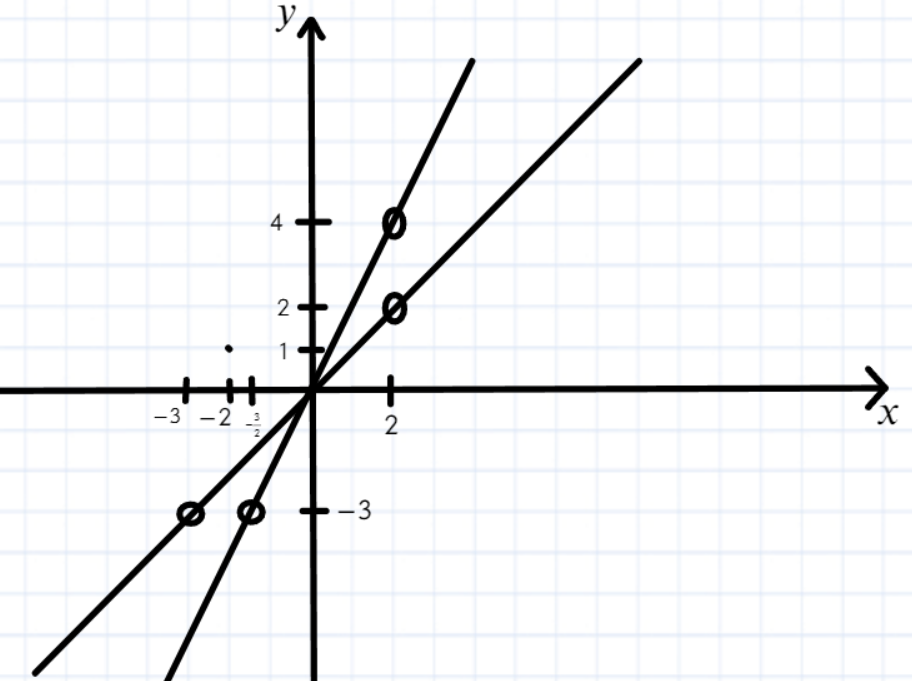
\includegraphics[scale=0.35]{gr7-82.png}}
\end{figure}\newpage\noindent
83. $\cfrac{((x^2-4)^2+y^2+2y+1)(y^2-4xy+3x^2)}{xy-2y+2x-4}=0\Leftrightarrow
\begin{cases}
((x^2-4)^2+y^2+2y+1)(y^2-4xy+3x^2)=0,\\
xy-2y+2x-4\neq0.
\end{cases}$\\$\Leftrightarrow
\begin{cases}
\left[\begin{array}{l}
(x^2-4)^2+(y+1)^2=0,\\
y(y-x)+3x(x-y)=0,
\end{array}\right.\\
y(x-2)+2(x-2)\neq0.
\end{cases}\Leftrightarrow
\begin{cases}
\left[\begin{array}{l}
\begin{cases}
x^2-4=0,\\
y+1=0.
\end{cases}\\
(y-x)(y-3x)=0,
\end{array}\right.\\
(x-2)(y+2)\neq0.
\end{cases}\Leftrightarrow
\begin{cases}
\left[\begin{array}{l}
\begin{cases}
x=2,\\
y=-1.
\end{cases}\\
\begin{cases}
x=-2,\\
y=-1.
\end{cases}\\
y=x,\\
y=3x,
\end{array}\right.\\
x\neq2,\\
y\neq-2.
\end{cases}$
\begin{figure}[ht!]
\center{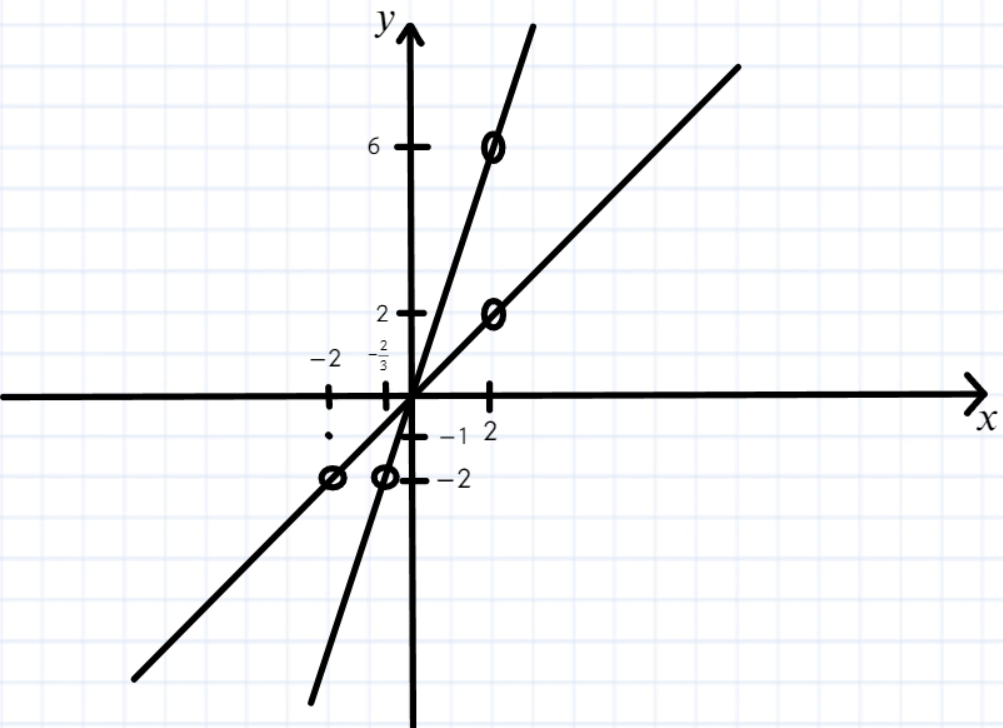
\includegraphics[scale=0.35]{gr7-83.png}}
\end{figure}\\
84. а) $y=\cfrac{x^2-2x}{2-x}+4=\cfrac{x(x-2)}{2-x}+4=\begin{cases} 4-x,\\ x\neq 2.\end{cases}$\\
\begin{figure}[ht!]
\center{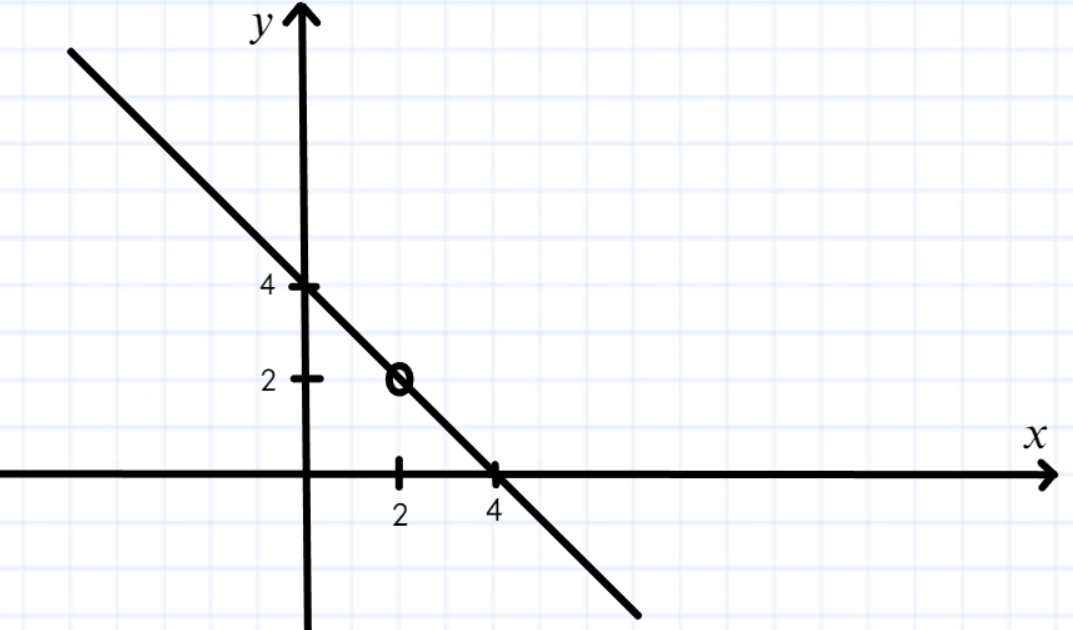
\includegraphics[scale=0.35]{gr7-84.png}}
\end{figure}\\
б) При положительных $x$ функция принимает значения $(-\infty;2)\cup(2;4).$\\
в) Эта прямая не будет иметь общих точек с графиком функции, если она параллельна прямой $y=4-x$ или если она проходит через выколотую точку $(2;2).$ Пусть это прямая $y=kx+b.$ В первом случае её угловой коэффициент равен $-1,$ значит $-1=-1+b,\ b=0,$ то есть это функция $y=-x.$ Во втором случае $\begin{cases} -1=k+b,\\ 2=2k+b.\end{cases}\Leftrightarrow
\begin{cases} -3=-k,\\ b=2-2k.\end{cases}\Leftrightarrow
\begin{cases} k=3,\\ b=-4.\end{cases},$ то есть прямая задана уравнением $y=3x-4.$\newpage\noindent
85. а) $y=\cfrac{x^2-3x}{3-x}+1=\cfrac{x(x-3)}{3-x}+1=\begin{cases} 1-x,\\ x\neq 3.\end{cases}$\\
\begin{figure}[ht!]
\center{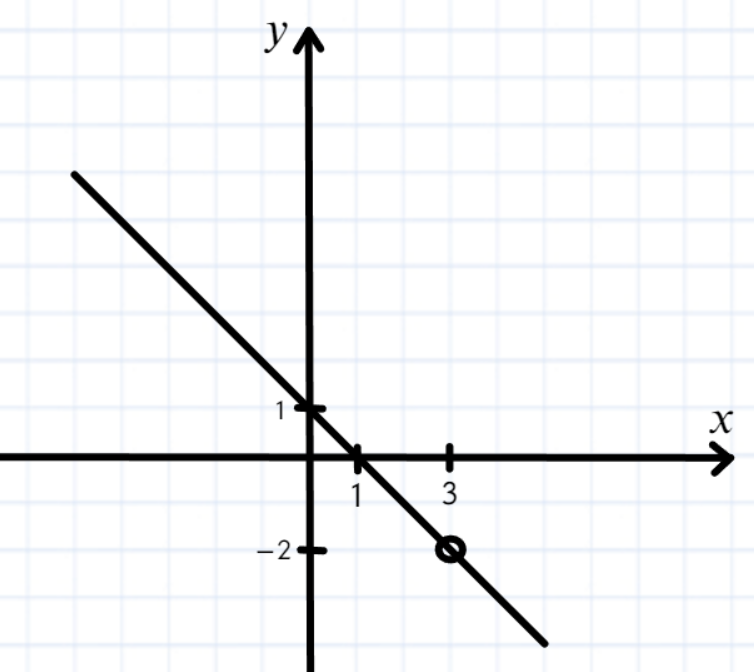
\includegraphics[scale=0.35]{gr7-85.png}}
\end{figure}\\
б) При положительных $x$ функция принимает значения $(-\infty;-2)\cup(-2;1).$\\
в) Эта прямая не будет иметь общих точек с графиком функции, если она параллельна прямой $y=1-x$ или если она проходит через выколотую точку $(3;-2).$ Пусть это прямая $y=kx+b.$ В первом случае её угловой коэффициент равен $-1,$ значит $-1=2+b,\ b=-3,$ то есть это функция $y=-x-3.$ Во втором случае $\begin{cases} -2=3k+b,\\ -1=-2k+b.\end{cases}\Leftrightarrow
\begin{cases} -1=5k,\\ b=2k-1.\end{cases}\Leftrightarrow
\begin{cases} k=-\cfrac{1}{5},\\ b=-\cfrac{7}{5}.\end{cases},$ то есть прямая задана уравнением $y=-\cfrac{1}{5}x-\cfrac{7}{5}.$\\
86. Найдём точку пересечения: $4x+3a=2x+4a,\ 2x=a,\ x=\cfrac{a}{2},\ y=2\cdot\cfrac{a}{2}+4a=5a.$ Если $5a=4,$ то $a=\cfrac{4}{5}.$\\
87. $y=\cfrac{x^2+2x}{|x|}=\cfrac{x(x+2)}{|x|}=\begin{cases} x+2,\ x>0,\\ -x-2,\ x<0.\end{cases}$\\
\begin{figure}[ht!]
\center{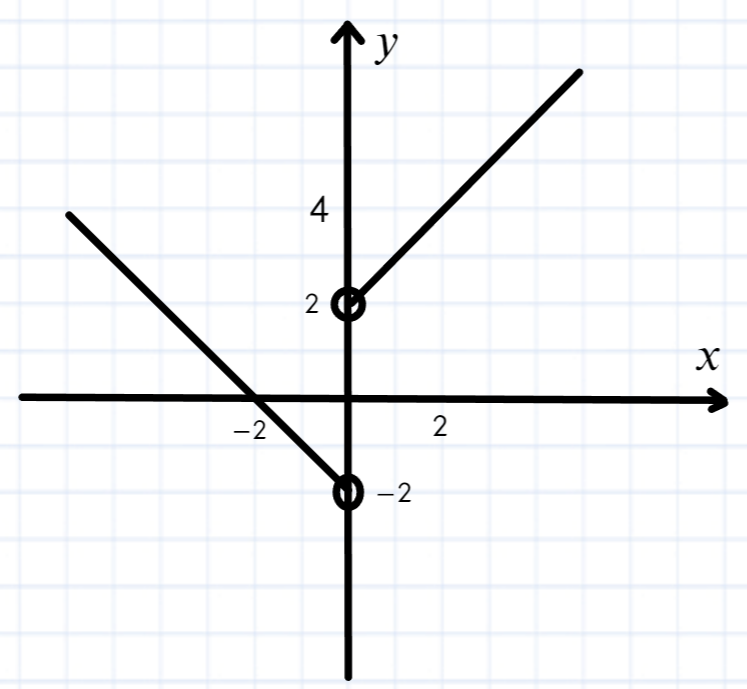
\includegraphics[scale=0.35]{gr7-87.png}}
\end{figure}\newpage\noindent
88. $y=\cfrac{4-x^2}{x+2}-1=\cfrac{(2-x)(2+x)}{x+2}-1=\begin{cases} 1-x,\\ x\neq-2.\end{cases}$\\
\begin{figure}[ht!]
\center{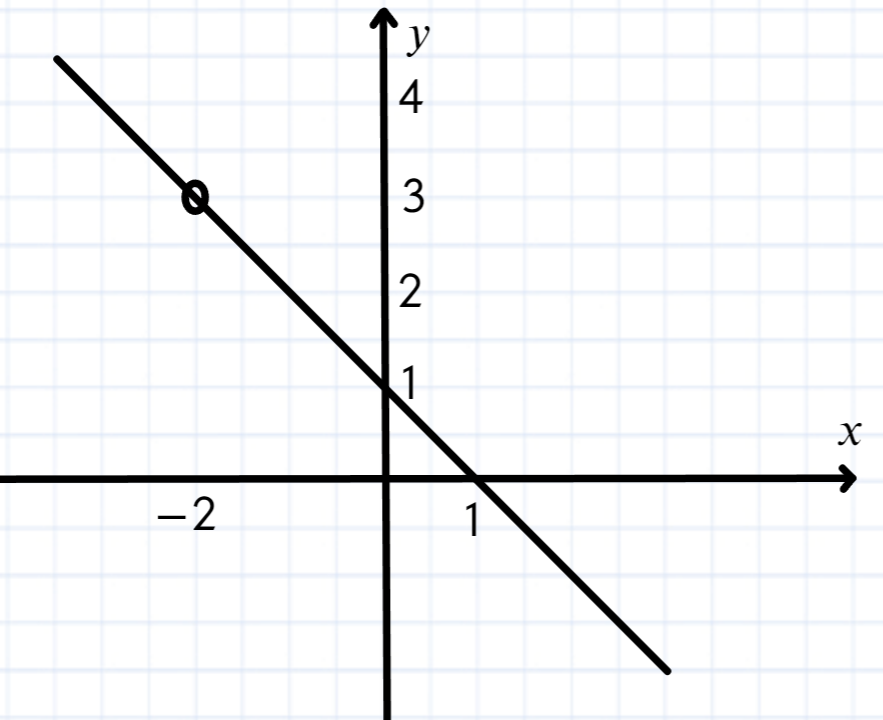
\includegraphics[scale=0.35]{gr7-88.png}}
\end{figure}\\
По графику определим подходящие значения 1, 2 и 4.\\
89. а) Подставим $x=0,$ тогда $y=0+d=d.$ Так как график этой функции пересекает ось ординат ниже оси абсцисс, получаем условие $d<0.$\\
б) Подставим координаты этой точки: $d=k+d,$ откуда $k=0,$ что соответствует горизонтальной прямой. Значит, график функции через эту точку не проходит.\\
90. Расстояние $AB$ всегда равно $(x+1)-(x-3)=4.$ Расстояние $BC$ может быть равно либо $(2x+3)-(x-3)=x+6,$ либо $(x-3)-(2x+3)=-x-6.$ В первом случае $x+6=4,\ x=-2,$ а во втором --- $-x-6=4,\ x=-10.$\\
91. Расстояние $AB$ всегда равно $(x+1)-(x-3)=4.$ Расстояние $AC$ может быть равно либо $(2x+3)-(x+1)=x+2,$ либо $(x+1)-(2x+3)=-x-2.$ В первом случае $x+2=4,\ x=2,$ а во втором --- $-x-2=4,\ x=-6.$\\
92. $y=\cfrac{2x^3+x^2-2x-1}{1-x^2}=\cfrac{x^2(2x+1)-(2x+1)}{1-x^2}=\cfrac{(2x+1)(x^2-1)}{1-x^2}=-2x-1,\ x\neq\pm1.$
$$\begin{tikzpicture}[scale=0.2]
\tikzset {line01/.style={line width =0.5pt}}
\tikzset{line02/.style={line width =1pt}}
\tikzset{line03/.style={dashed,line width =0.5pt}}
%\filldraw [black] (0,0) circle (1pt);
\draw [->] (-10,0) -- (10,0);
\draw [->] (0,-10) -- (0,10);
\draw[line01] (-5,9) -- (4,-9);
\draw (10.2,0.7) node {\scriptsize $x$};
\draw (-1.2,-1.3) node {\scriptsize $-1$};
\draw (1.2,0.7) node {\scriptsize $1$};
\draw (0.4,1) node {\scriptsize $1$};
\draw (-1.1,-3) node {\scriptsize $-3$};
%\draw (0.7,6) node {\scriptsize $6$};
%\draw (-5.5,-2) node {\scriptsize $-6$};
\draw[line03] (-1,0) -- (-1,1);
\draw[line03] (-0.9,1) -- (0,1);
\draw[line03] (1,0) -- (1,-3);
\draw[line03] (1,-3) -- (0,-3);

\draw (0.7,10.2) node {\scriptsize $y$};
\draw (1,-3) circle (10pt);
\draw (-1,1) circle (10pt);
\end{tikzpicture}$$
93. $y=\cfrac{x^3-x^2-x+1}{1-x^2}=\cfrac{x^2(x-1)-(x-1)}{1-x^2}=\cfrac{(x-1)(x^2-1)}{1-x^2}=1-x,\ x\neq\pm1.$
$$\begin{tikzpicture}[scale=0.2]
\tikzset {line01/.style={line width =0.5pt}}
\tikzset{line02/.style={line width =1pt}}
\tikzset{line03/.style={dashed,line width =0.5pt}}
%\filldraw [black] (0,0) circle (1pt);
\draw [->] (-10,0) -- (10,0);
\draw [->] (0,-10) -- (0,10);
\draw[line01] (-7,8) -- (4,-3);
\draw (10.2,0.7) node {\scriptsize $x$};
\draw (-1.2,-1.3) node {\scriptsize $-1$};
\draw (1.2,0.9) node {\scriptsize $1$};
\draw (0.4,2) node {\scriptsize $2$};

%\draw (0.7,6) node {\scriptsize $6$};
%\draw (-5.5,-2) node {\scriptsize $-6$};
\draw[line03] (-1,0) -- (-1,2);
\draw[line03] (-0.9,2) -- (0,2);


\draw (0.7,10.2) node {\scriptsize $y$};
\draw (1,0) circle (10pt);
\draw (-1,2) circle (10pt);
\end{tikzpicture}$$\\
94. $\cfrac{(4+x(2y-x)-y^2)(x^2+y^2-2(x+y-1))}{3x+y+xy+3}=0\Leftrightarrow$\\$
\begin{cases}

(4+x(2y-x)-y^2)(x^2+y^2-2(x+y-1))=0,\\
3x+y+xy+3\neq0.
\end{cases}\Leftrightarrow$\\$
\begin{cases}
\left[\begin{array}{l}
4+2xy-x^2-y^2=0,\\
x^2+y^2-2x-2y+2=0.
\end{array}\right.\\
x(y+3)+y+3\neq0.
\end{cases}\Leftrightarrow
\begin{cases}
\left[\begin{array}{l}
4=(y-x)^2,\\
(x-1)^2+(y-1)^2=0.
\end{array}\right.\\
(x+1)(y+3)\neq0.
\end{cases}\Leftrightarrow
\begin{cases}
\left[\begin{array}{l}
\begin{cases}
x=1,\\
y=1.
\end{cases}\\
y=2+x,\\
y=-2+x,
\end{array}\right.\\
x\neq-1,\\
y\neq-3.
\end{cases}$
\begin{figure}[ht!]
\center{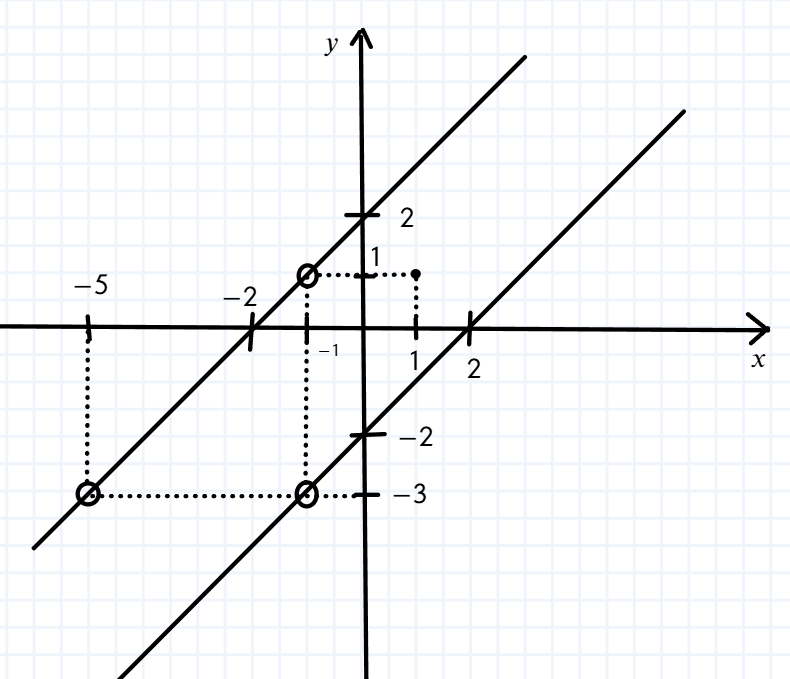
\includegraphics[scale=0.35]{gr7-97.png}}
\end{figure}\\
95. $\cfrac{(4-x(2y+x)-y^2)}{(2x-2y+xy-4)(x^2+y^2-2(x+y-1))}=0\Leftrightarrow$\\$
\begin{cases}

4-x(2y+x)-y^2=0,\\
(2x-2y+xy-4)(x^2+y^2-2(x+y-1))\neq0.
\end{cases}\Leftrightarrow$\\$
\begin{cases}
4-2xy-x^2-y^2=0,\\
x^2+y^2-2x-2y+2\neq0,\\
x(y+2)-2(y+2)\neq0.
\end{cases}\Leftrightarrow
\begin{cases}
4=(y+x)^2,\\
(x-1)^2+(y-1)^2\neq0,\\
(x-2)(y+2)\neq0.
\end{cases}\Leftrightarrow
\begin{cases}
\left[\begin{array}{l}
y=2-x,\\
y=-2-x,
\end{array}\right.\\
(x;y)\neq (1;1),\\
x\neq2,\\
y\neq-2.
\end{cases}$
\begin{figure}[ht!]
\center{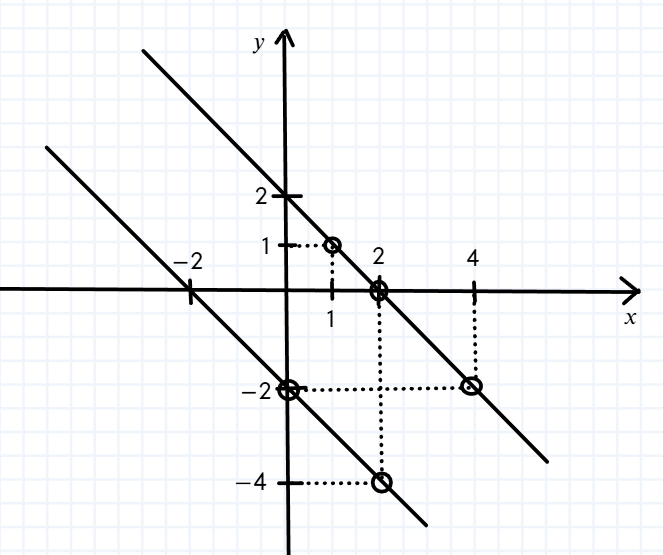
\includegraphics[scale=0.35]{gr7-98.png}}
\end{figure}
\newpage
